\chapter{Virtual Private Cloud (VPC)}\label{ch:vpc}

Amazon VPC allows for AWS resources to be launched in a virtual network that has been custom defined and configured.
This virtual network is similar to a traditional network which operates within your own physical data center, with the
added benefits of the scalable AWS infrastructure~\parencite{amazon2022what}.
A VPC can have multiple assigned subnets, which are a range of IP addresses accessible in the VPC\@.
This chapter of the report will detail the creation of an Elastic IP address, a VPC, subnets, an internet gateway, and
route tables.

\section{Elastic IP Address}\label{sec:elastic-ip-address}

Before creating the VPC, an Elastic IP address must be created, which can then be allocated to the VPC\@.
To do this, the \textbf{Allocate Elastic IP address} button on the Elastic IP Addresses page must be clicked.

\begin{figure}[!htbp]
    \centering
    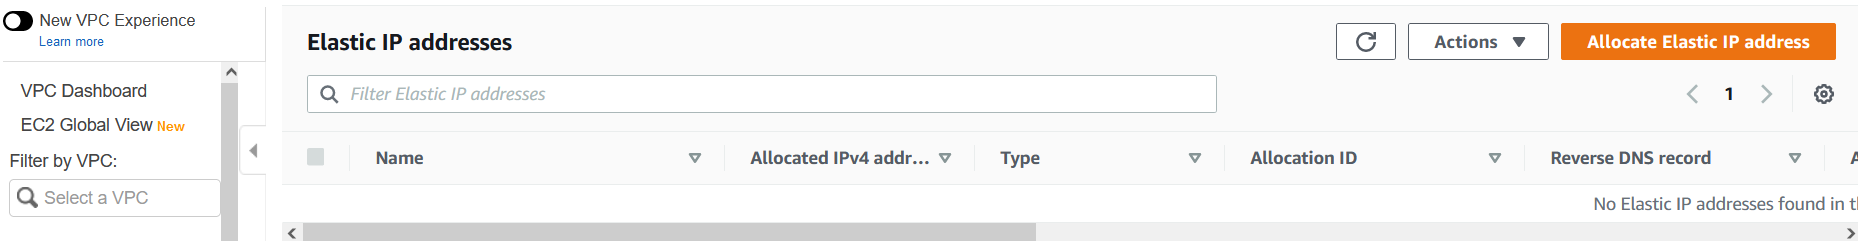
\includegraphics[width=150mm]{resources/vpc/blank_elastic}
    \caption{Elastic IP Addresses page.}
    \label{fig:blank-elastic}
\end{figure}

To configure the Elastic IP address, a Network Border Group must be selected, ensuring that this is the same as the
Availability Zone selected when configuring the VPC\@.
Once this has been set, and the remaining options are set to their default values, clicking the \textbf{Allocate} button
will create the Elastic IP address.

\clearpage
\begin{figure}[!htbp]
    \centering
    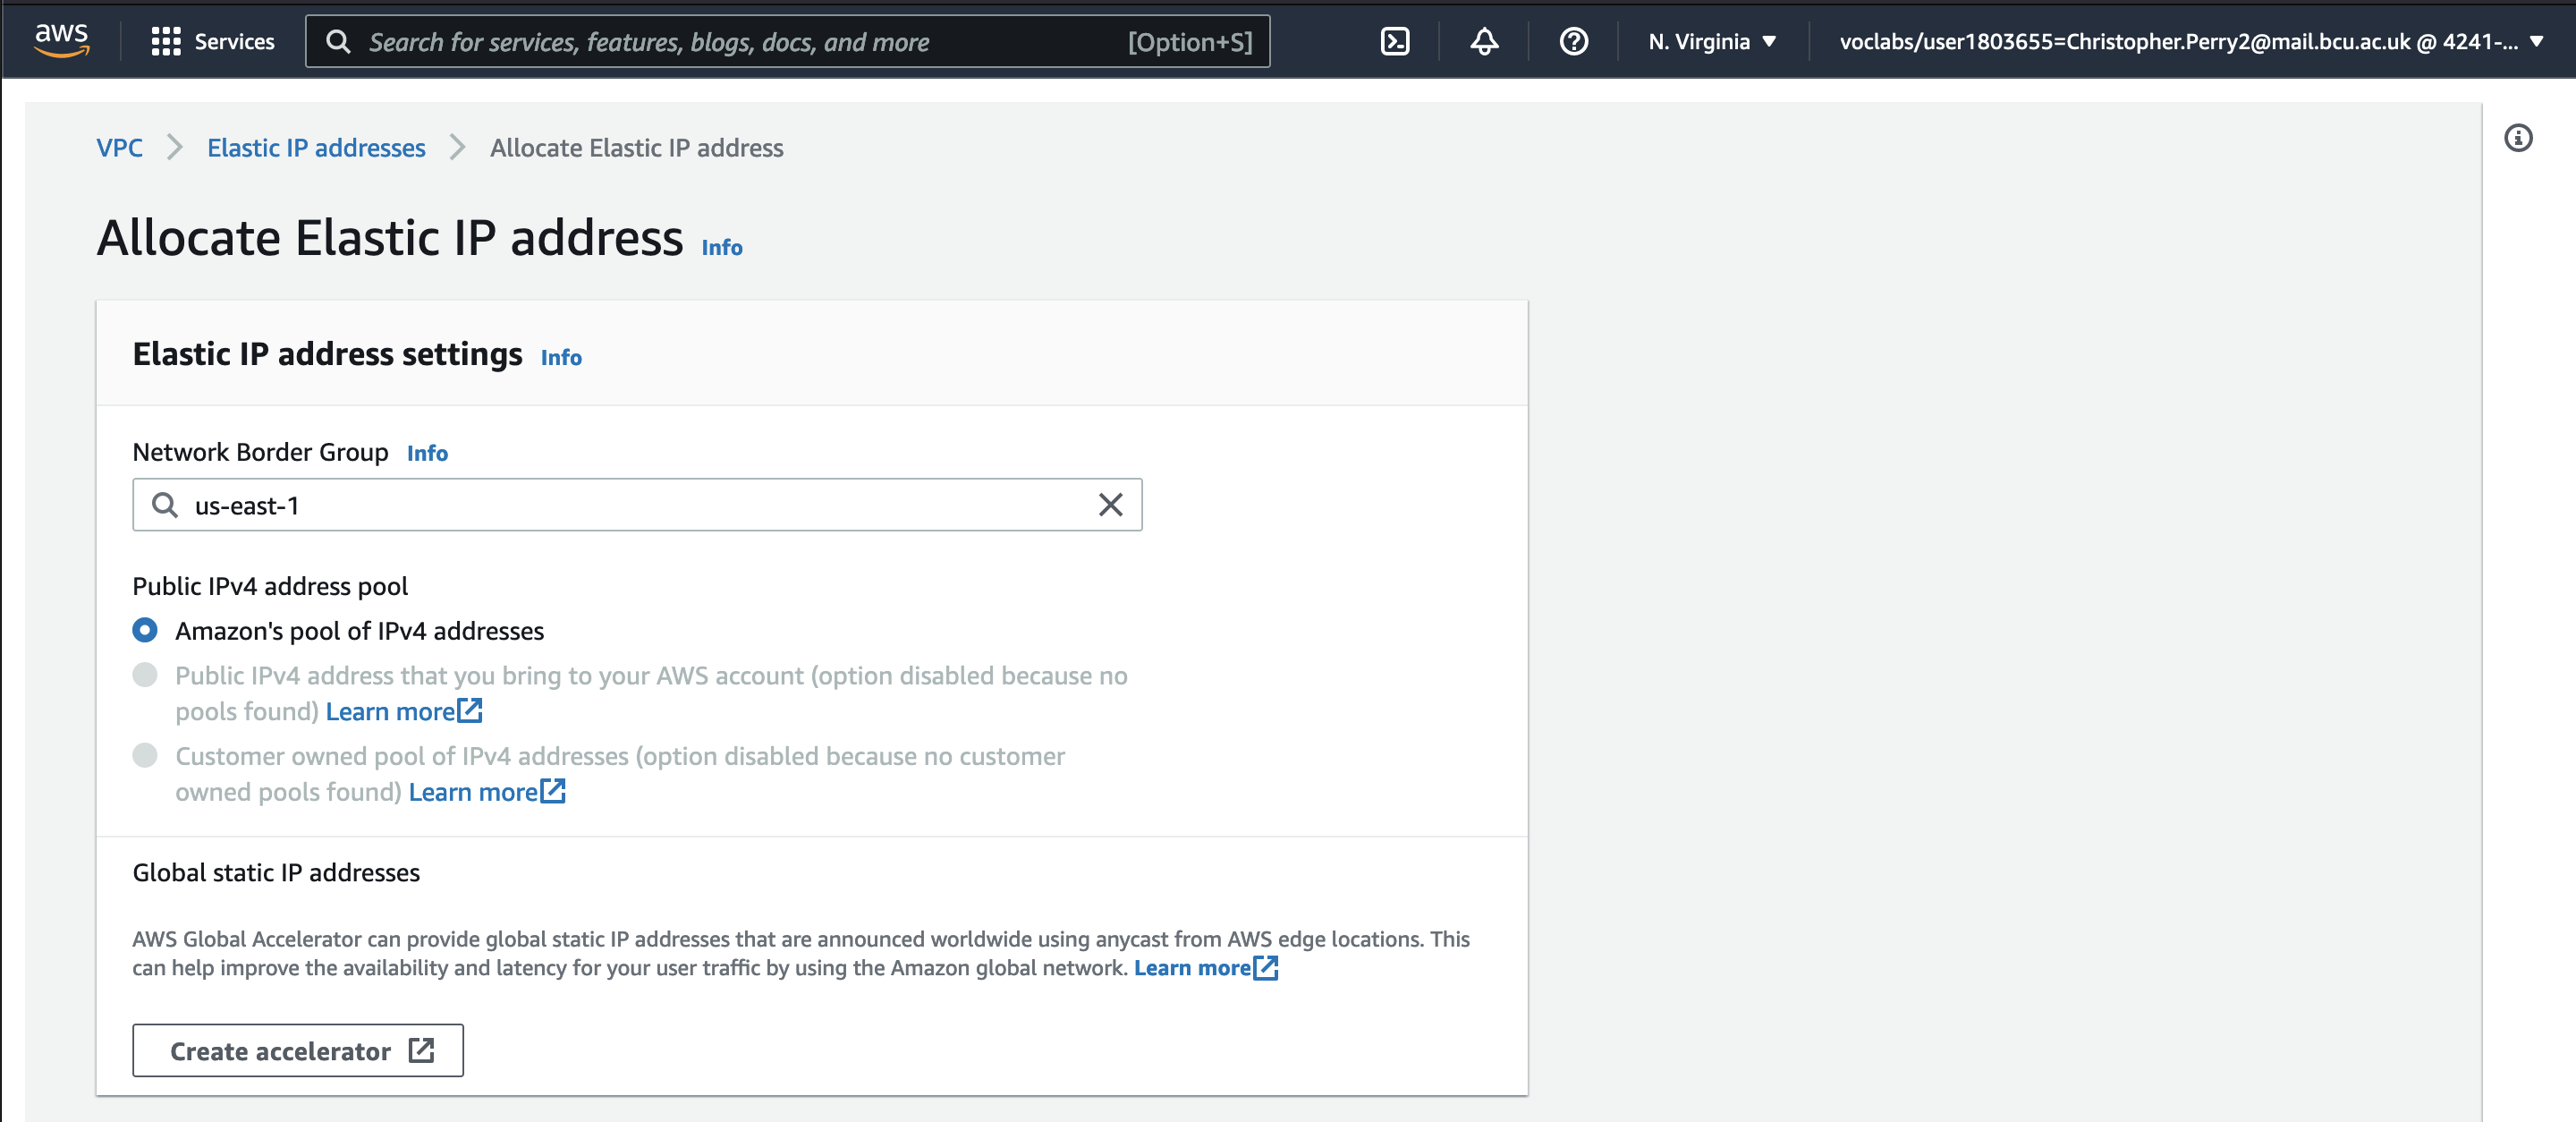
\includegraphics[width=150mm]{resources/vpc/vpc_elastic_ip_addresses}
    \caption{Configuring the Elastic IP address.}
    \label{fig:config-elastic}
\end{figure}

After this, the Elastic IP address created can be seen from the Elastic IP Addresses page.

\begin{figure}[!htbp]
    \centering
    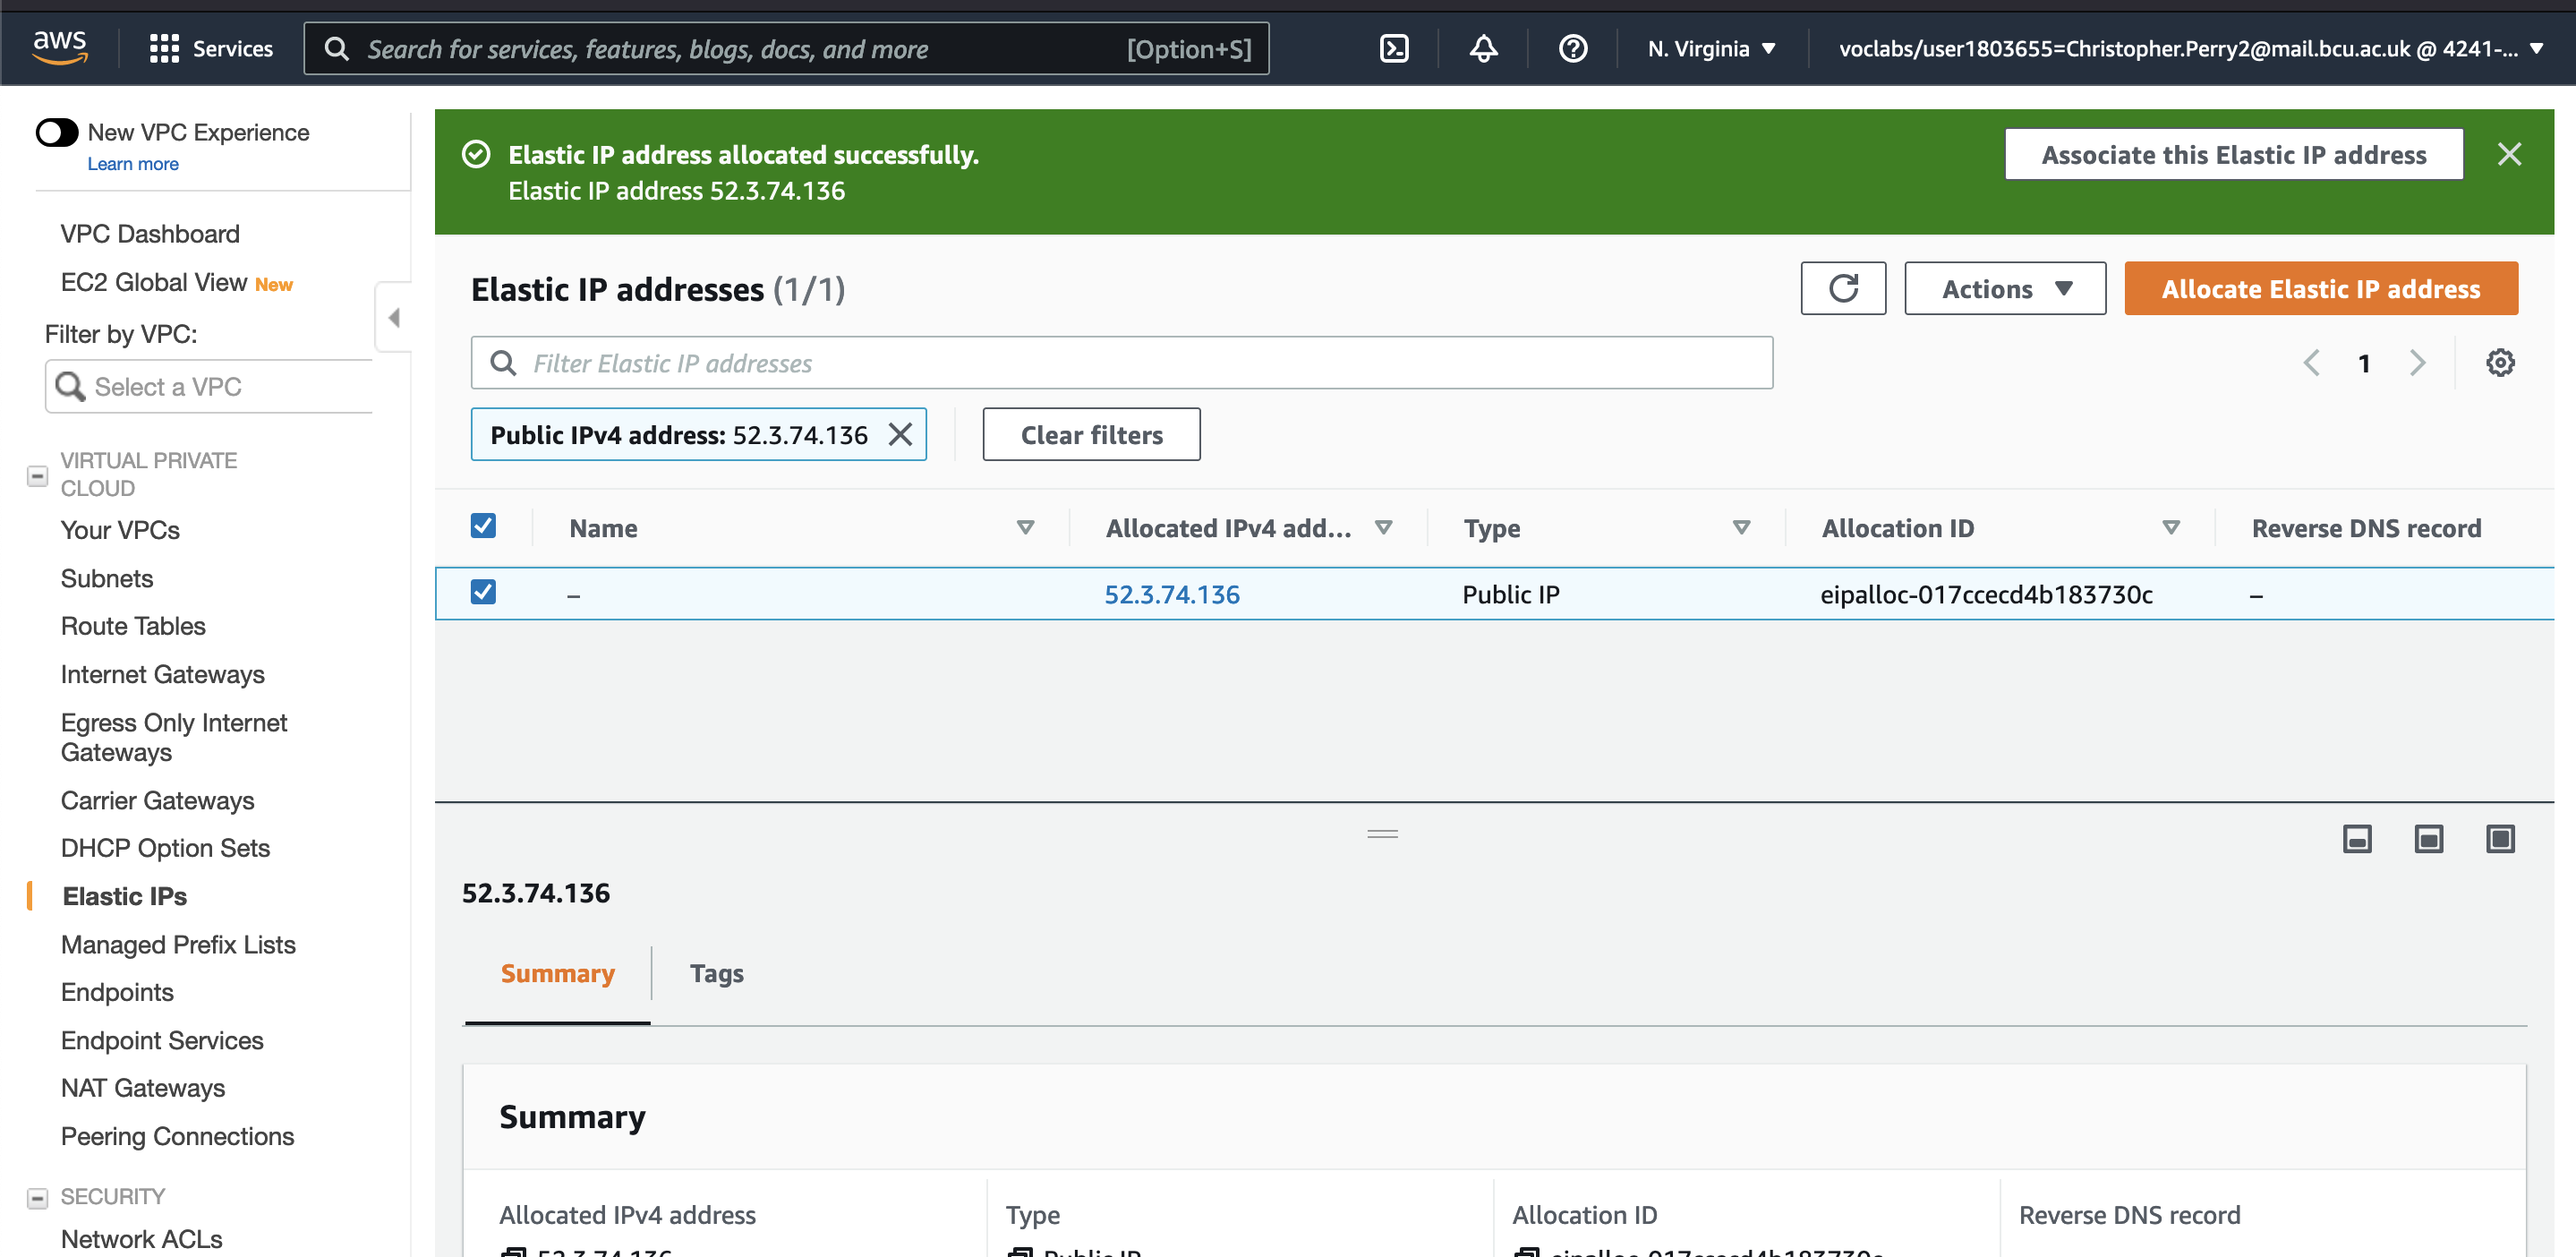
\includegraphics[width=150mm]{resources/vpc/elastic_ip_addresses}
    \caption{Created Elastic IP address.}
    \label{fig:elastic-ip-addresses}
\end{figure}

\clearpage
\section{VPC and Subnets}\label{sec:vpc-and-subnets}

The first step of migrating the web app to the cloud was creating a VPC to deploy and manage AWS resources for the app.
To do this, the VPC wizard must be used.
This is accessed by navigating to the VPC Management Console and then click the \textbf{Launch VPC Wizard} button, which
can be seen in Figure~\ref{fig:vpc-wizard}.

\begin{figure}[!htbp]
    \centering
    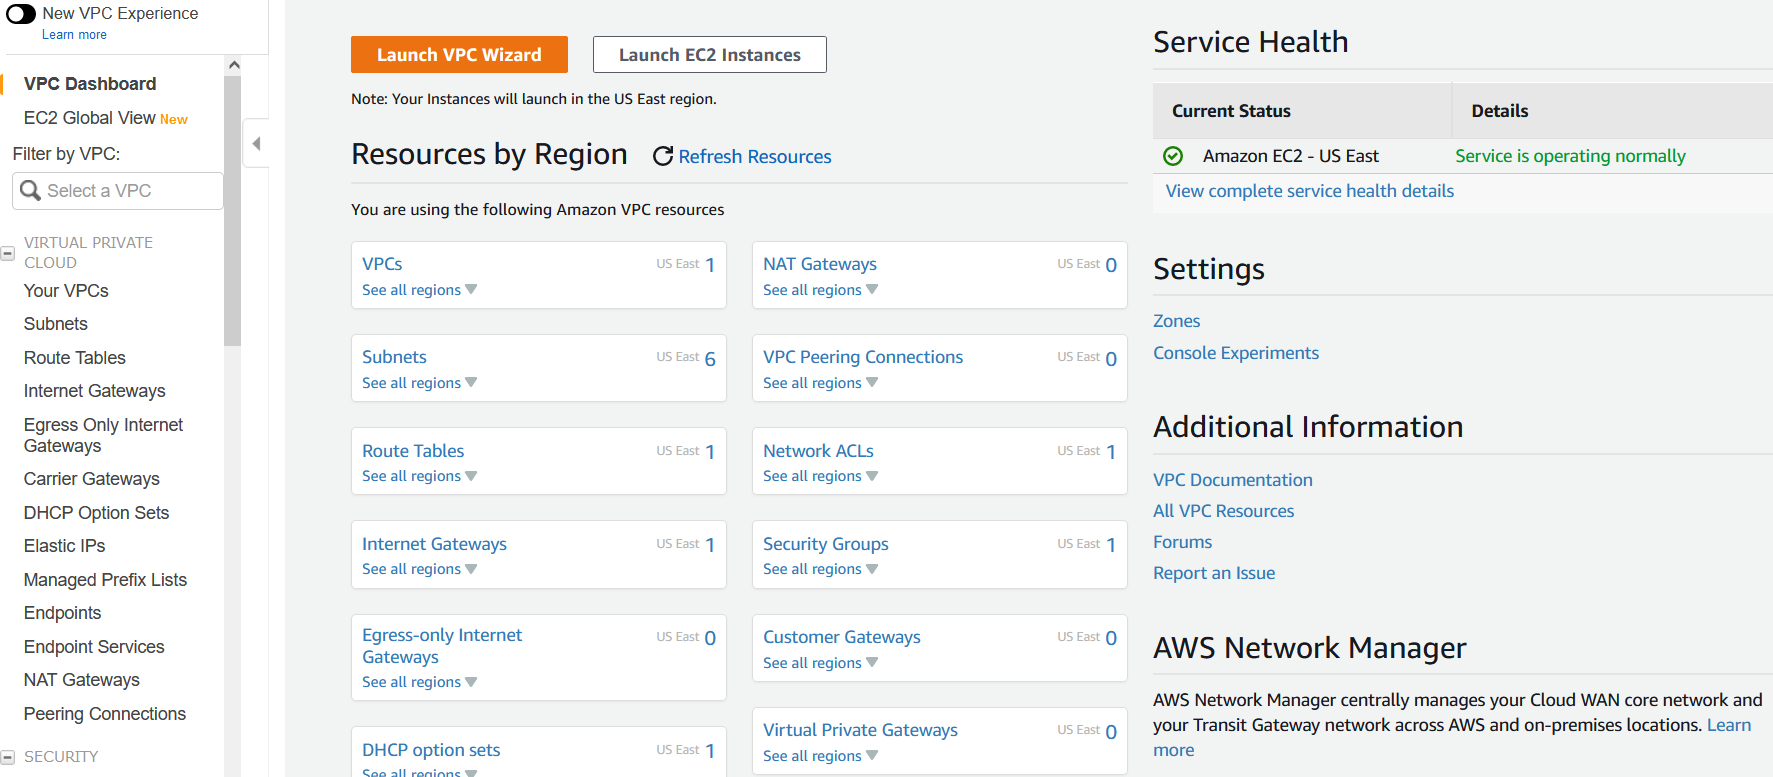
\includegraphics[width=150mm]{resources/vpc/vpc-dashboard}
    \caption{VPC Management Console.}
    \label{fig:vpc-wizard}
\end{figure}

The wizard presents us with step one of creating a VPC: selecting a VPC configuration.
There are several options for this, where each configuration has the following features:

\begin{itemize}
    \item VPC with a Single Public Subnet: Creates a /16 network with a /24 subnet where the subnet instances use
    Elastic IPs or Public IPs for internet access.
    \item VPC with Public and Private Subnets: Creates a /16 network and two /24 subnets where the public subnet
    instances use Elastic IPs for internet access and the private subnet instances use NAT for internet access.
    \item VPC with Public and Private Subnets and Hardware VPN Access: Creates a /16 network with two /24 subnets where
    one subnet is connected to the internet and another is connected to your personal network via a VPN\@.
    \item VPC with a Private Subnet Only and Hardware VPN Access: Creates a/16 network and a /24 subnet where the
    subnet is connected to your personal network via a VPN\@.
\end{itemize}

\clearpage
For the deployment of this web app, hardware VPN access is not necessary, so the VPC configuration with public and
private subnets was selected, as seen in Figure~\ref{fig:vpc-step-1}.

\begin{figure}[!htbp]
    \centering
    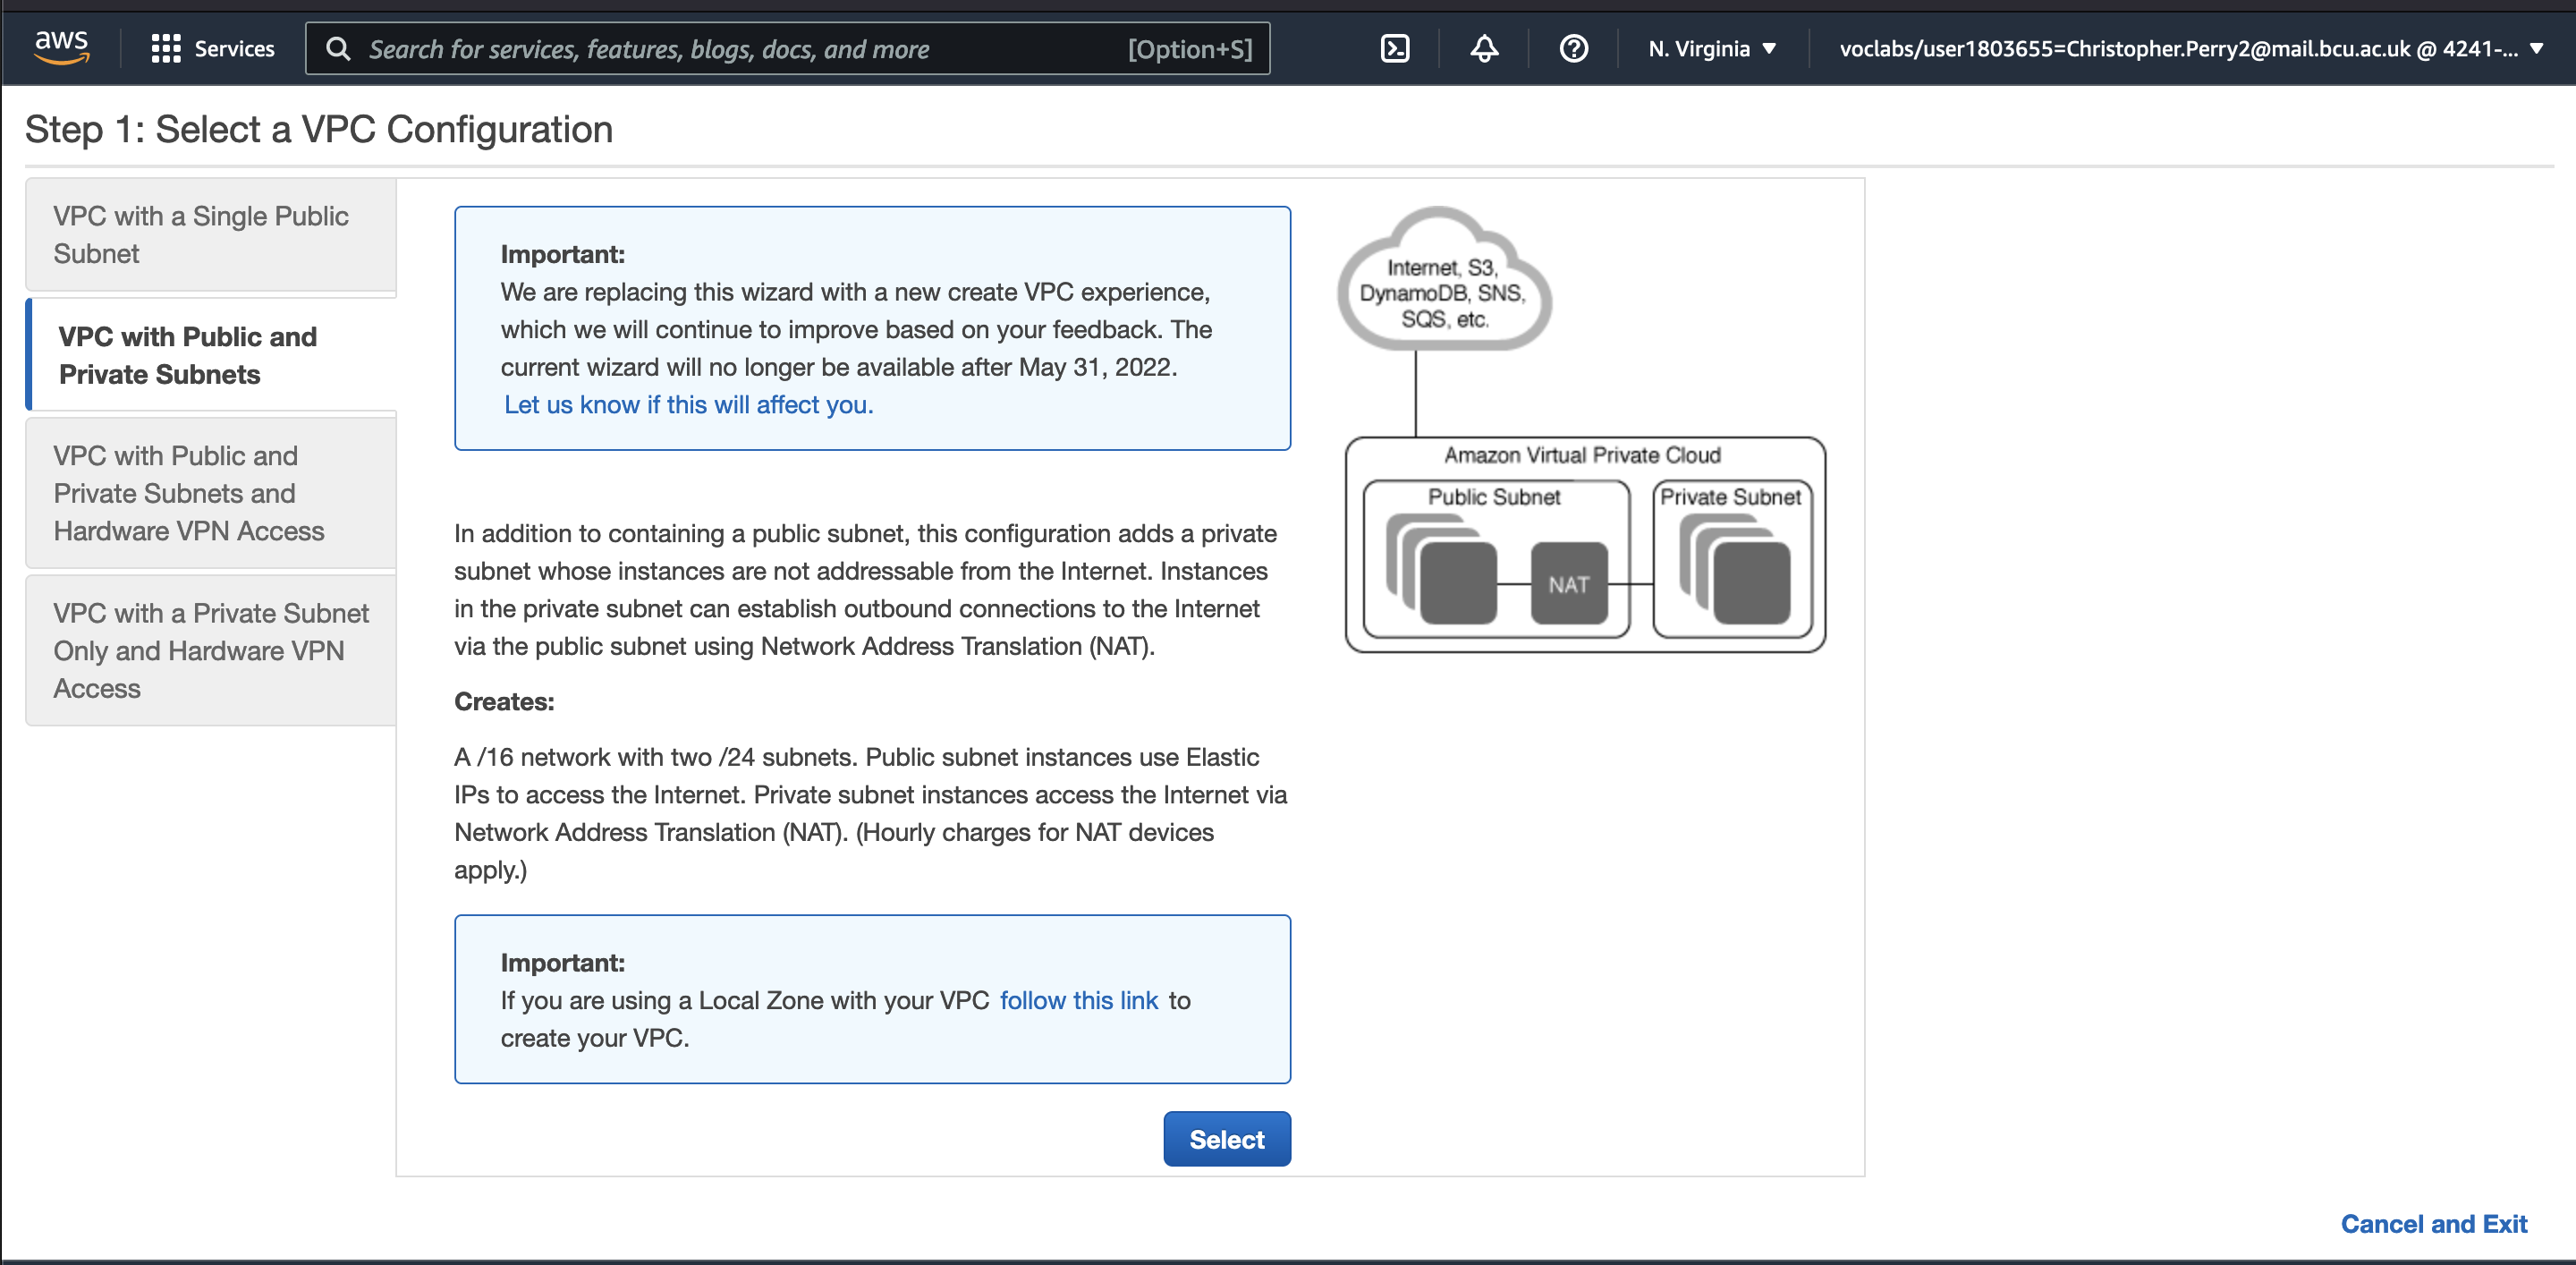
\includegraphics[width=115mm]{resources/vpc/step_1_select_a_vpc_configuration}
    \caption{Selecting a VPC configuration.}
    \label{fig:vpc-step-1}
\end{figure}

Following this, the specific details, such as the IP address block, of the selected configuration must be entered.
An IPv4 CIDR block of \mintinline{zsh}|10.0.0.0/16| was chosen as it provides a large amount of available IP addresses.
Additionally, no IPv6 CIDR block was configured and the VPC was named \mintinline{zsh}|Group4_VPC|.

Next, the public and private subnets were configured.
The public subnet was assigned an IPv4 CIDR of \mintinline{zsh}|10.0.0.0/24|, making 251 distinct IP addresses available
for the public subnet.
The availability zone of \mintinline{zsh}|us-east-1a| was chosen and the subnet was named
\mintinline{zsh}|Public subnet 1|.
The private subnet was assigned an IPv4 CIDR of \mintinline{zsh}|10.0.1.0/24|, making 251 distinct IP addresses
available for the private subnet as well.
The availability zone of \mintinline{zsh}|us-east-1a| was chosen and the subnet was named
\mintinline{zsh}|Private subnet 1|.

Lastly, the previously created Elastic IP Allocation ID was selected, and the remaining settings were left at their
default values.
Clicking the \textbf{Create VPC} button now will generate the VPC with the specified configurations.

\begin{figure}[!htbp]
    \centering
    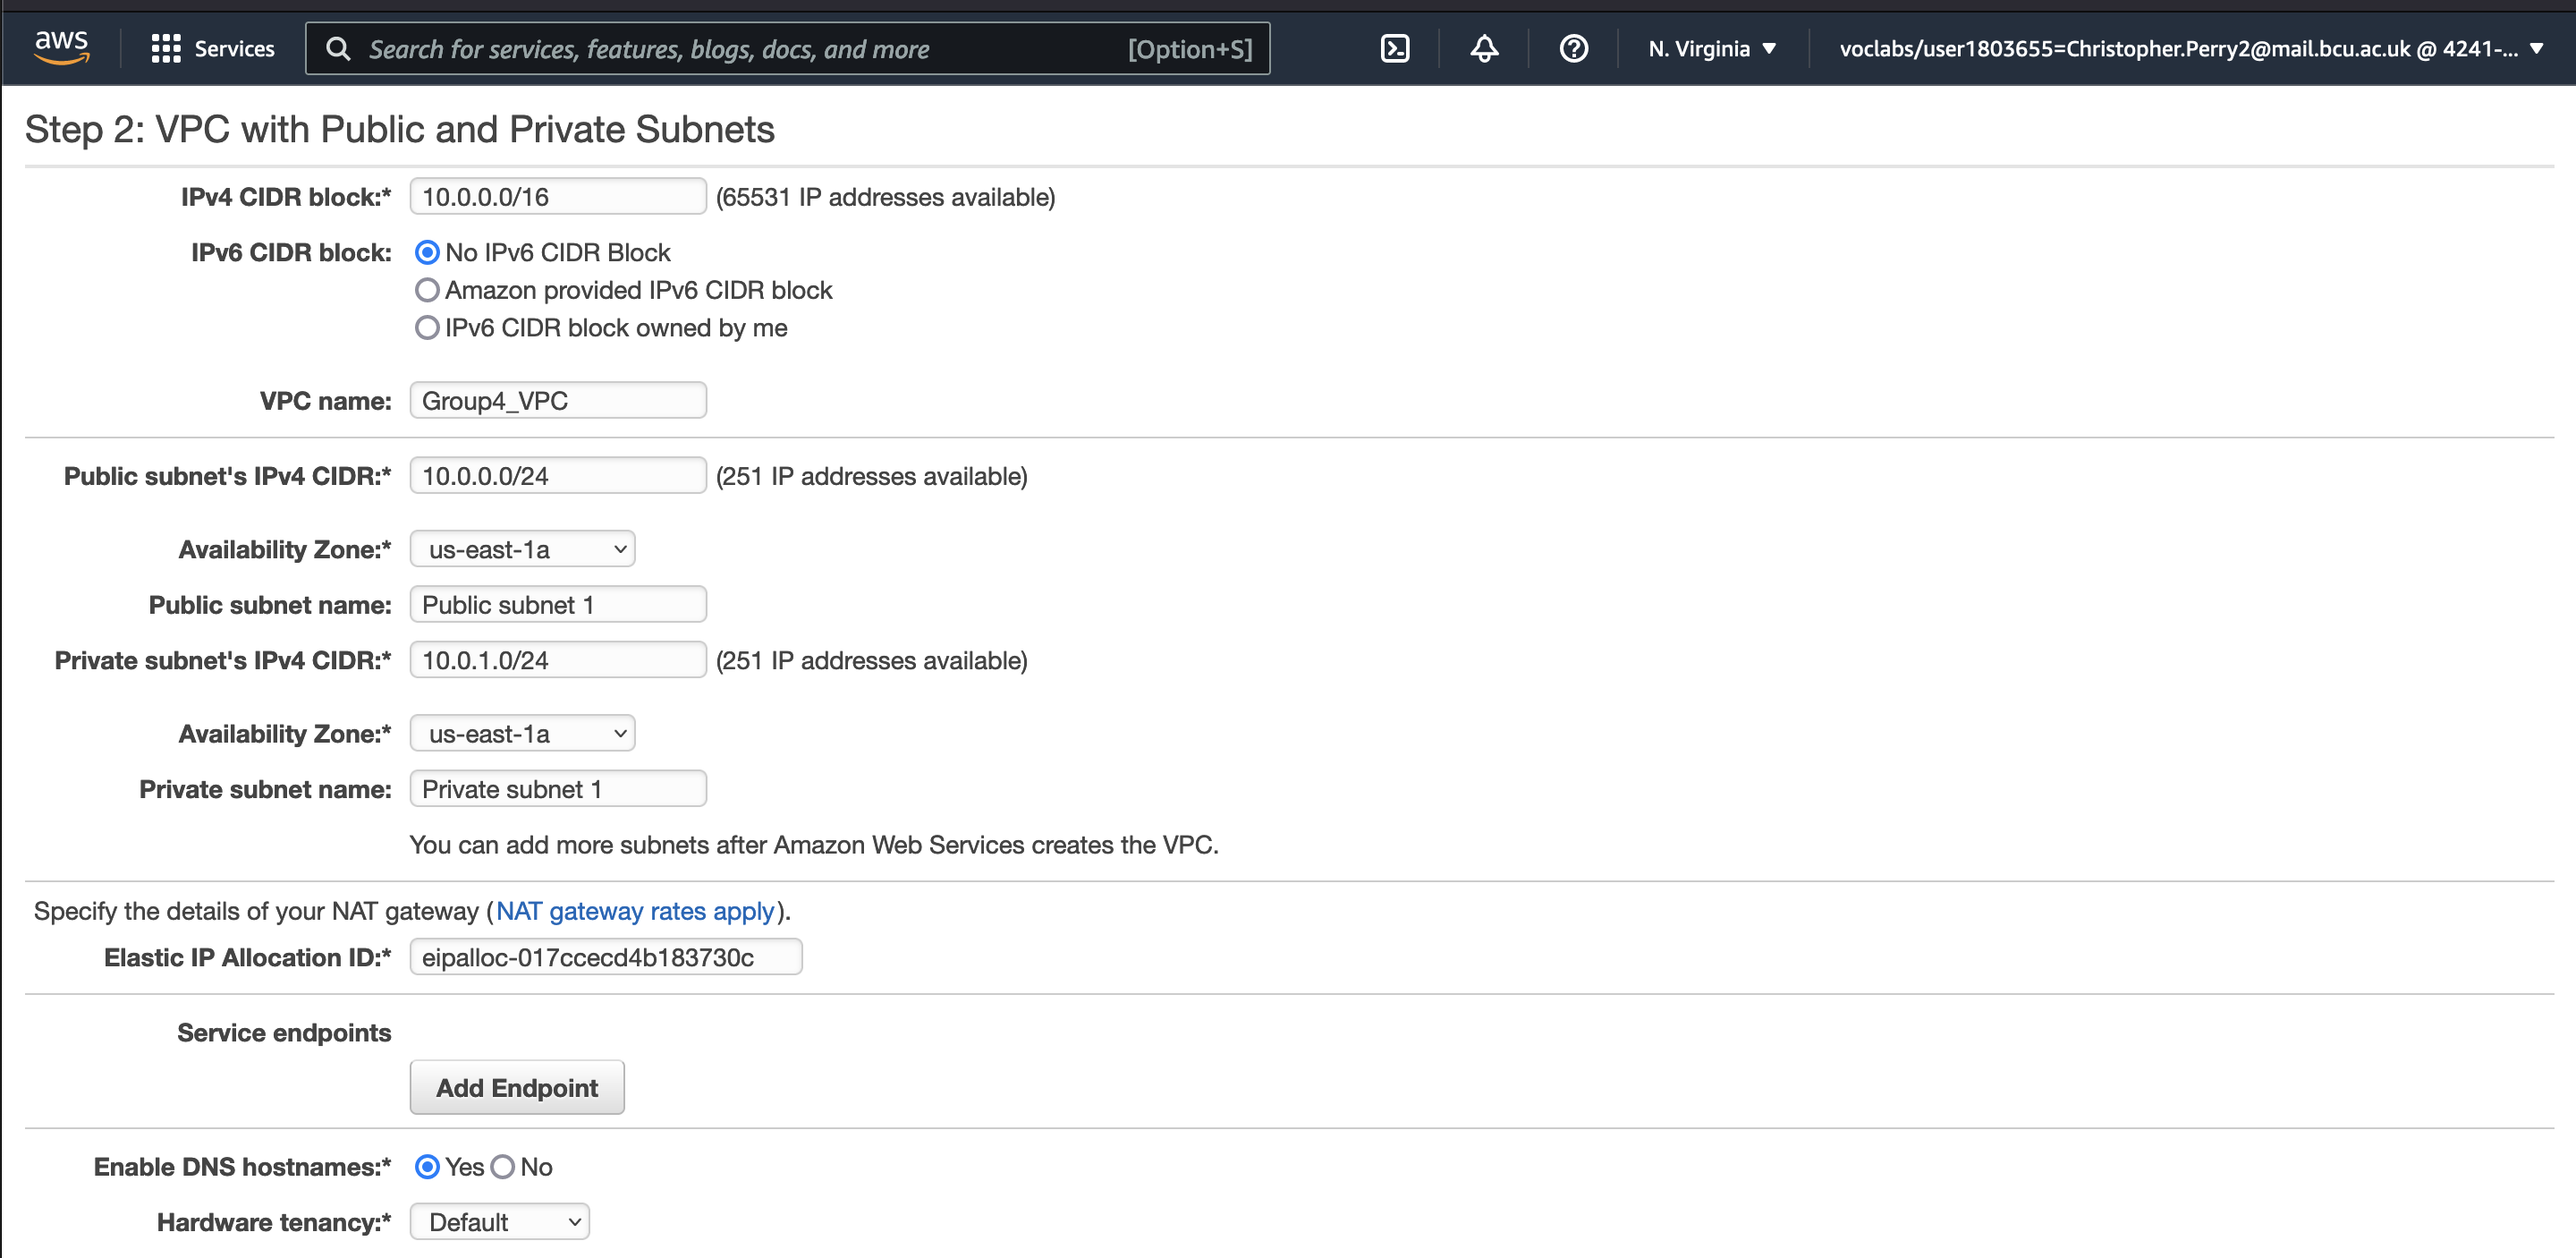
\includegraphics[width=115mm]{resources/vpc/step_2_vpc_with_public_and_private_subnets}
    \caption{Configuring VPC public and private subnets.}
    \label{fig:vpc-step-2}
\end{figure}

\clearpage
After this, AWS takes a few minutes to generate the VPC\@.

\begin{figure}[!htbp]
    \centering
    \subfloat{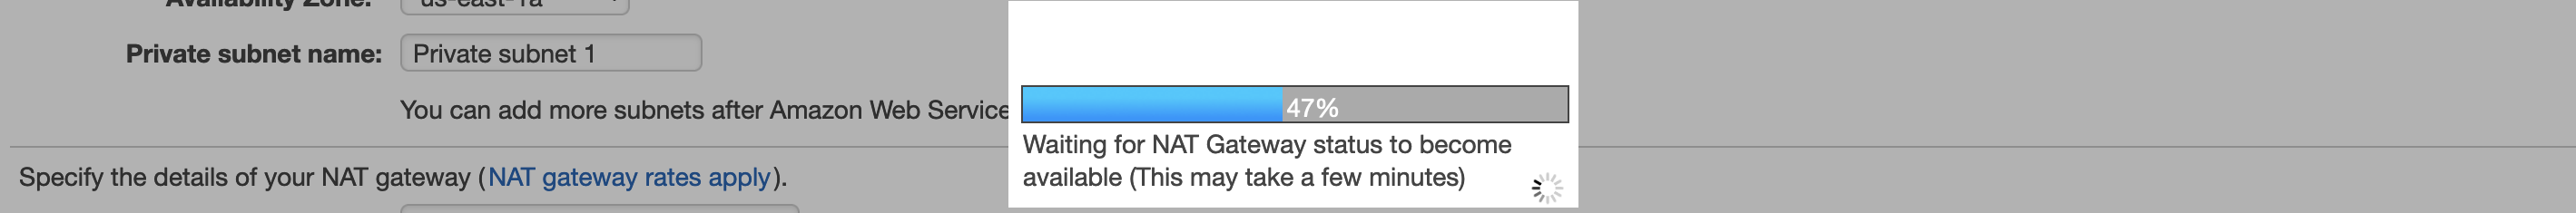
\includegraphics[width=150mm]{resources/vpc/step_3_create_vpc}}\hfill
    \subfloat{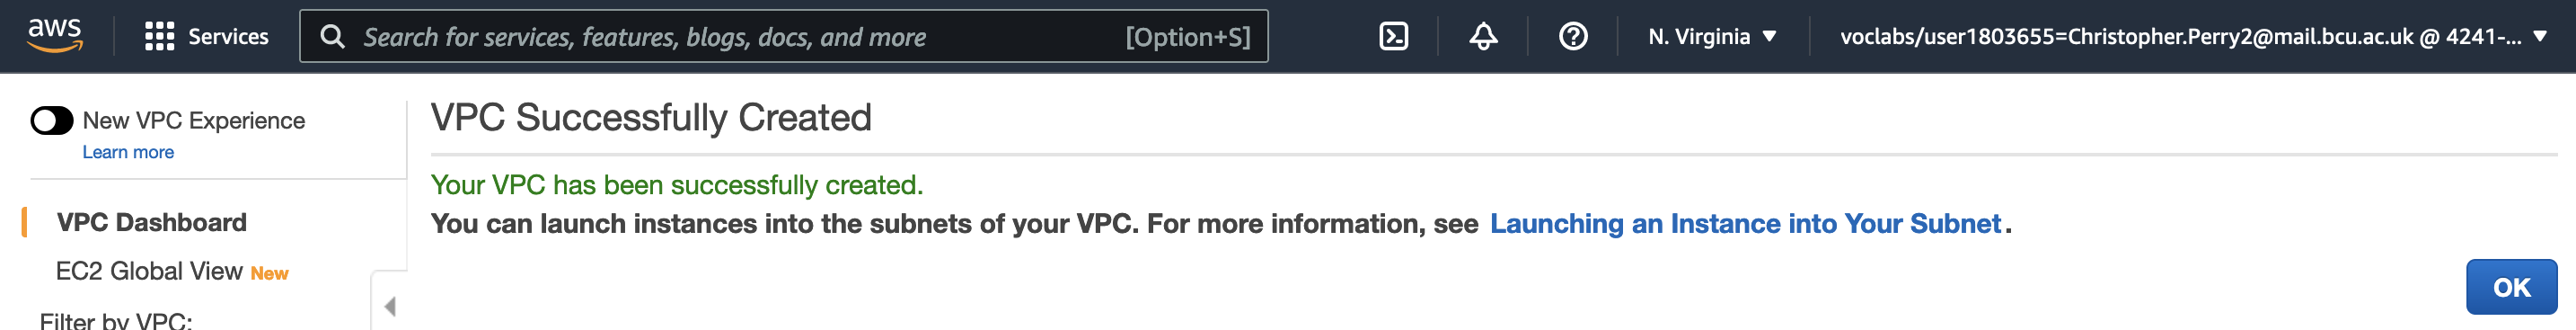
\includegraphics[width=150mm]{resources/vpc/vpc_successfully_created}}
    \caption{Generating the VPC.}
    \label{fig:vpc-step-3-and-4}
\end{figure}

Navigating from here to the Your VPCs page shows two available VPCs: the VPC created by the AWS sandbox
environment, which will not be used, and the VPC which has just been created, named \mintinline{zsh}|Group4_VPC|.

\begin{figure}[!htbp]
    \centering
    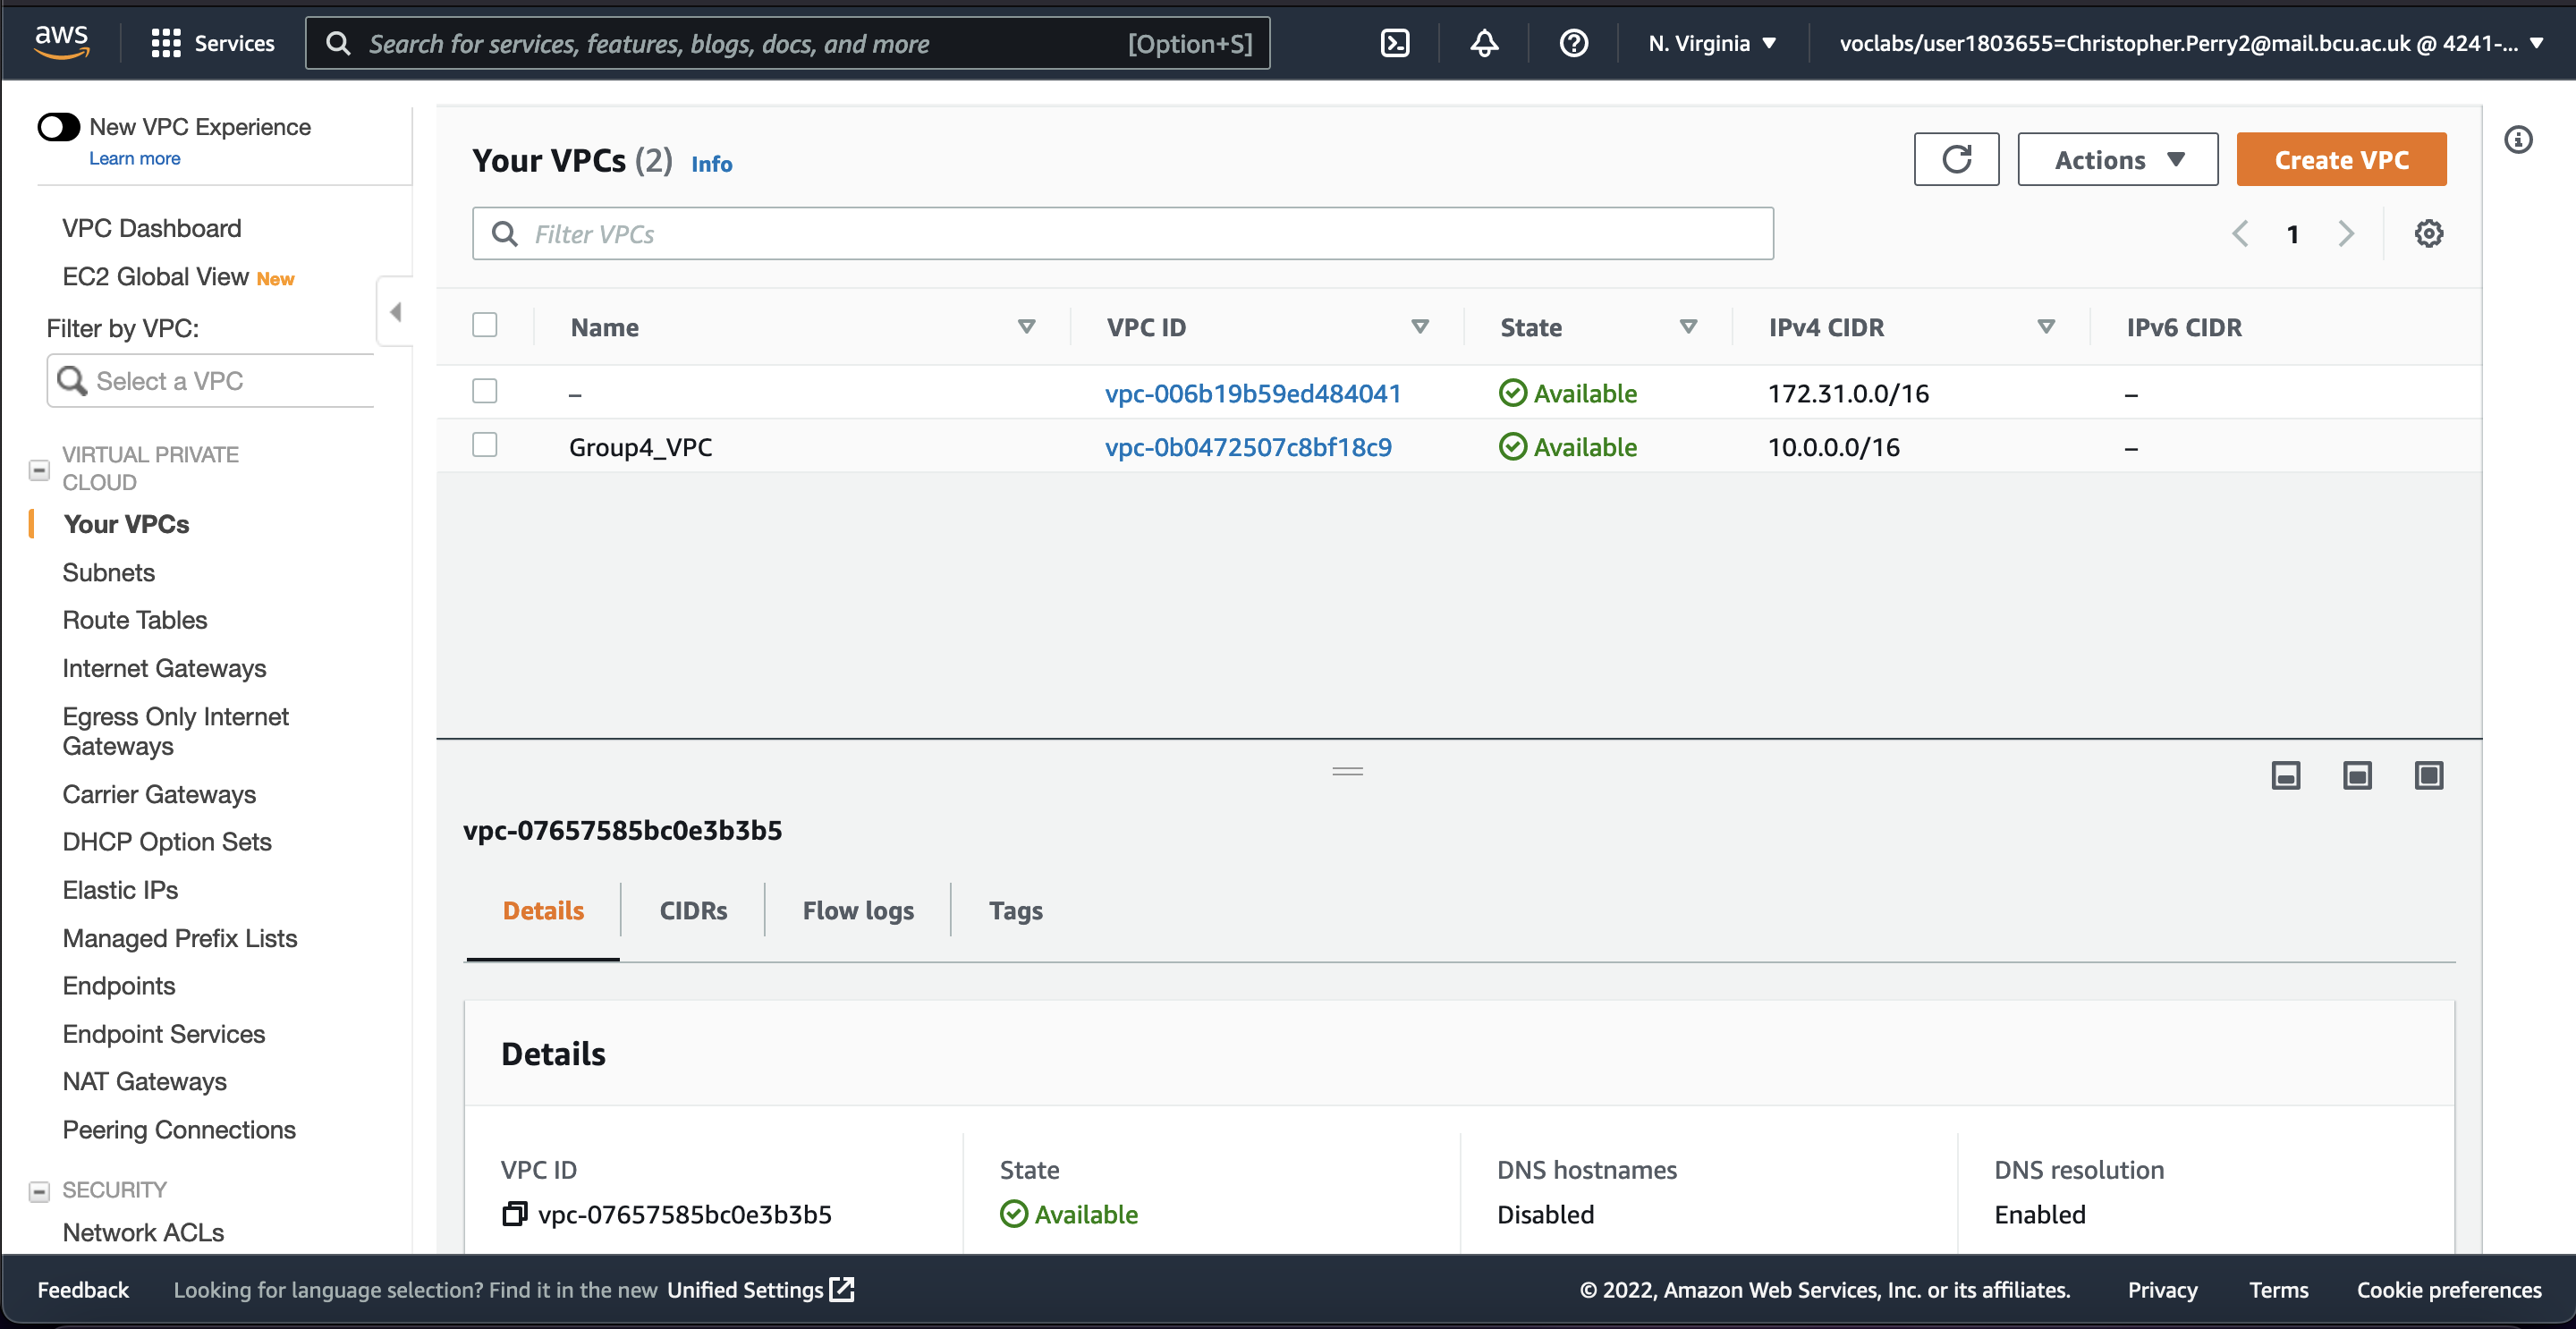
\includegraphics[width=150mm]{resources/vpc/your_vpcs}
    \caption{Your VPCs page.}
    \label{fig:vpc-step-5}
\end{figure}

\clearpage
\section{Internet Gateway}\label{sec:internet-gateway}

An internet gateway is required for resources, such as EC2, to be able to communicate with the internet, if the resource
has a public IP address~\parencite{amazon2022connect}.
To do this, navigate to the Internet Gateways page and click the \textbf{Create internet gateway} button.
Here, enter the internet gateway name, such as \mintinline{zsh}|Group4-Internet-Gateway|.

\begin{figure}[!htbp]
    \centering
    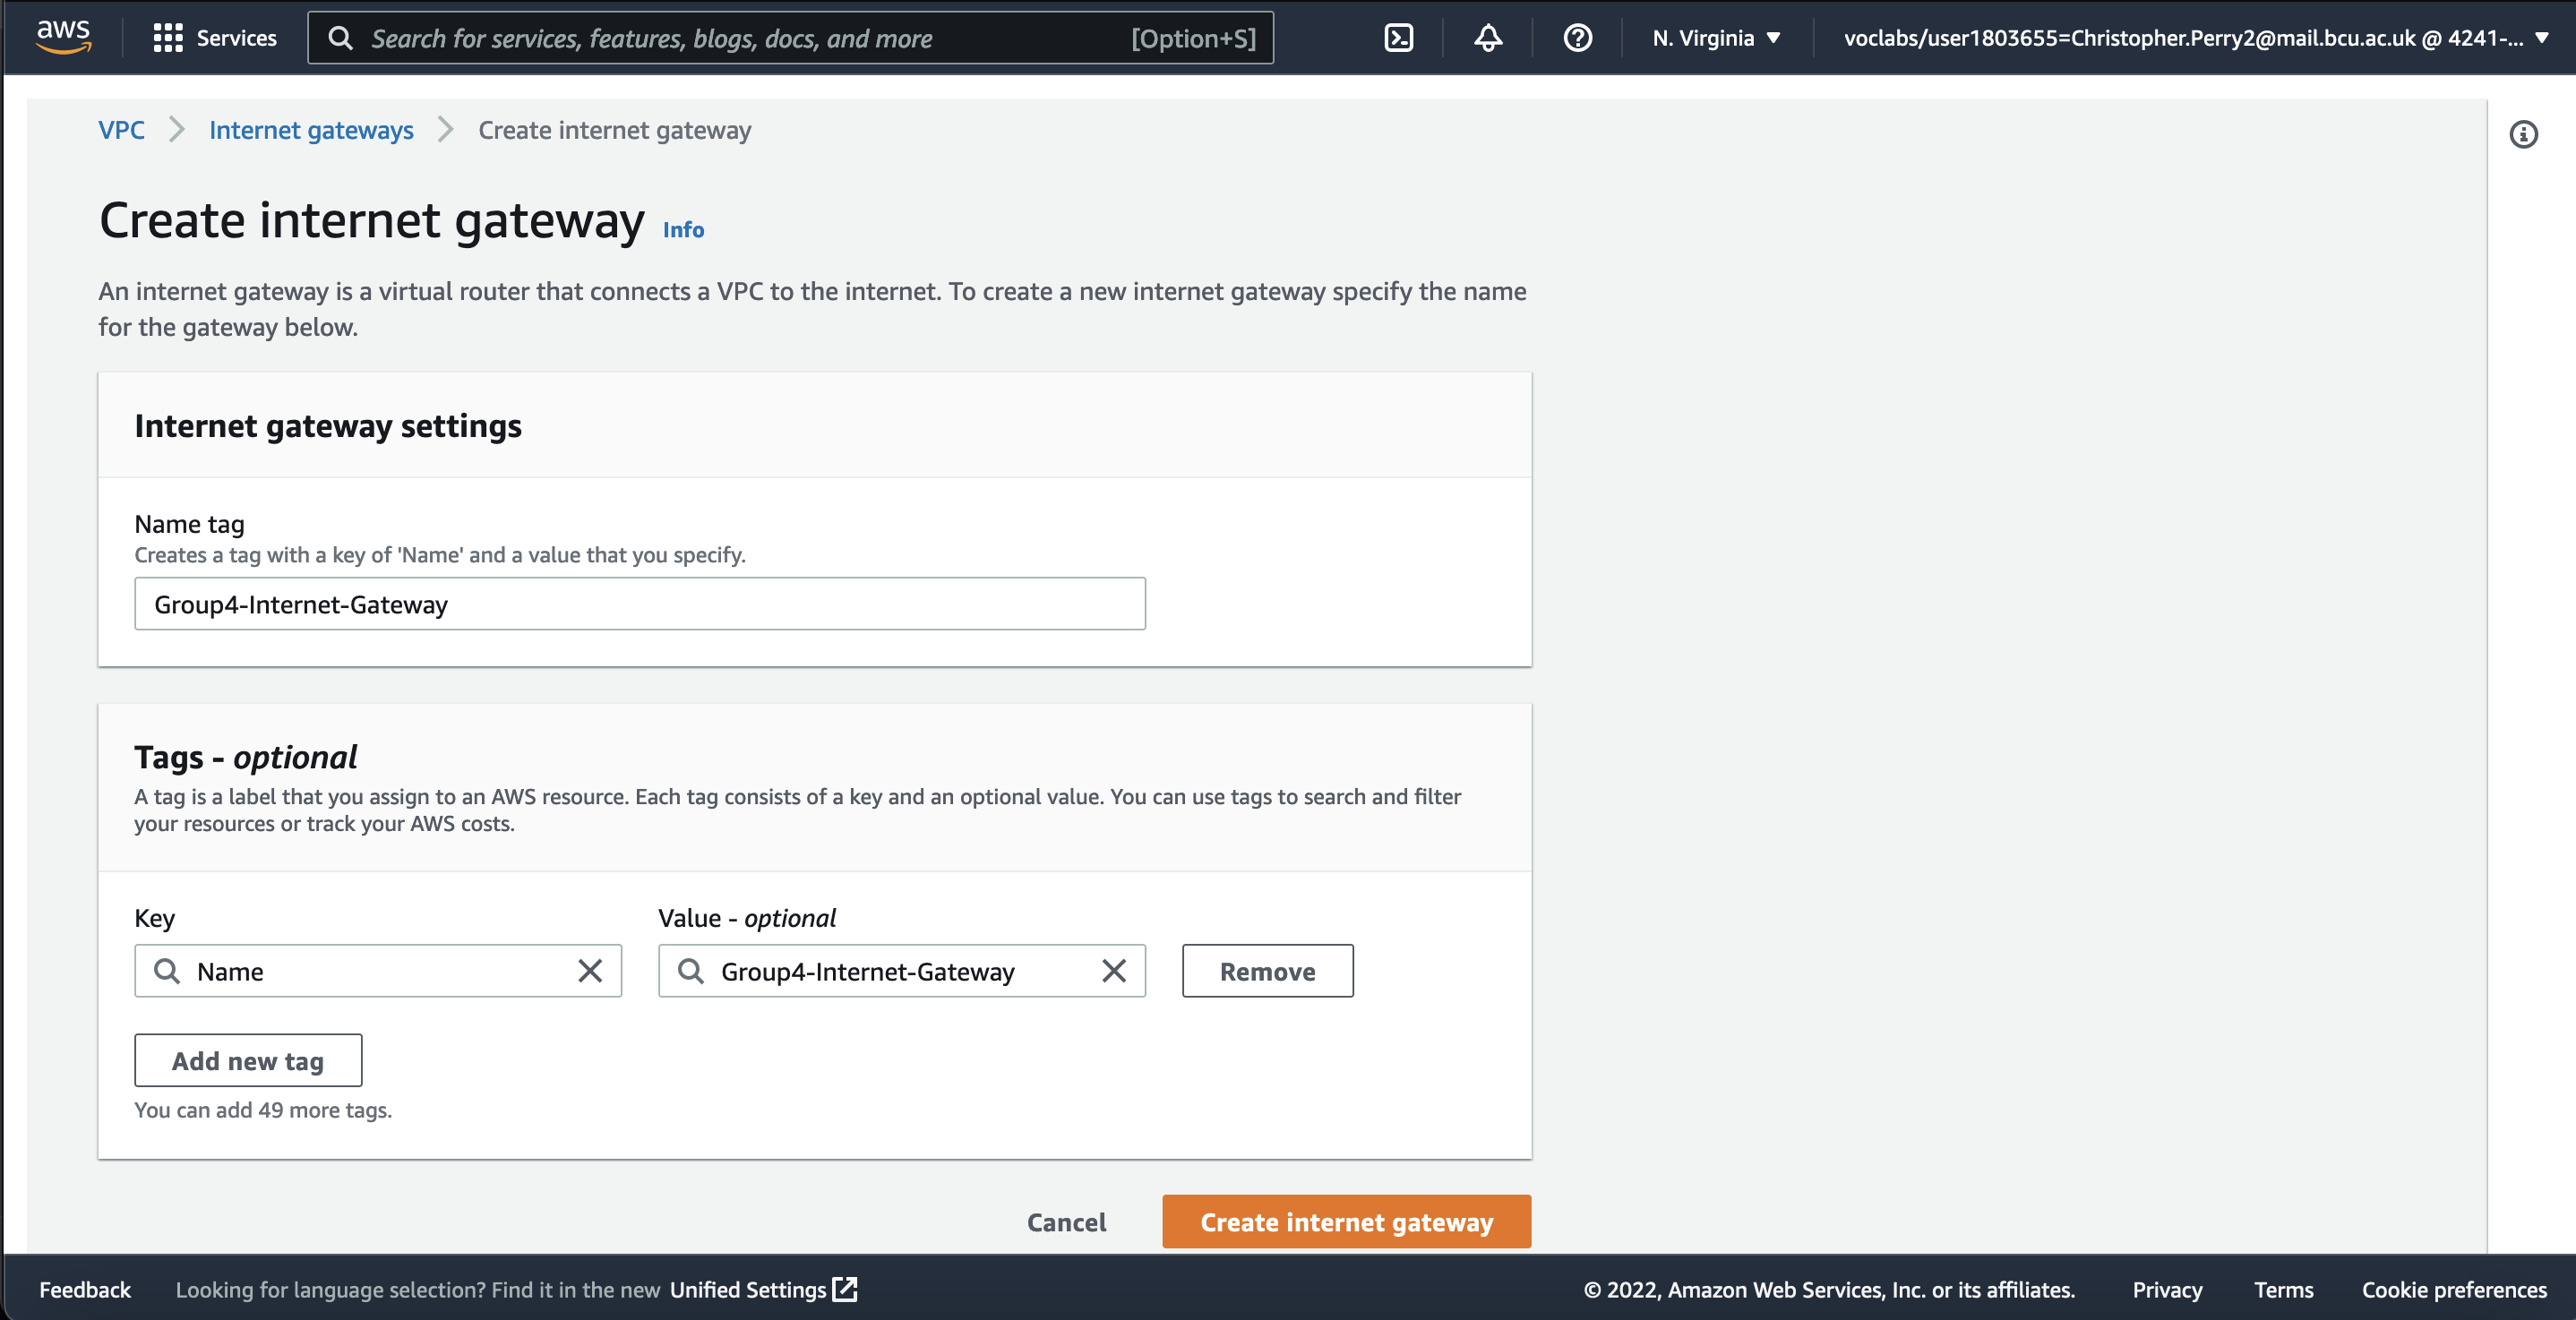
\includegraphics[width=150mm]{resources/vpc/internet-gateway-1}
    \caption{Creating an internet gateway.}
    \label{fig:internet-gateway-1}
\end{figure}

After entering the internet gateway name and clicking the \textbf{Create internet gateway} button, the newly created
internet gateway can be seen (as well as an automatically generated internet gateway for the default VPC, which will not
be used).

\begin{figure}[!htbp]
    \centering
    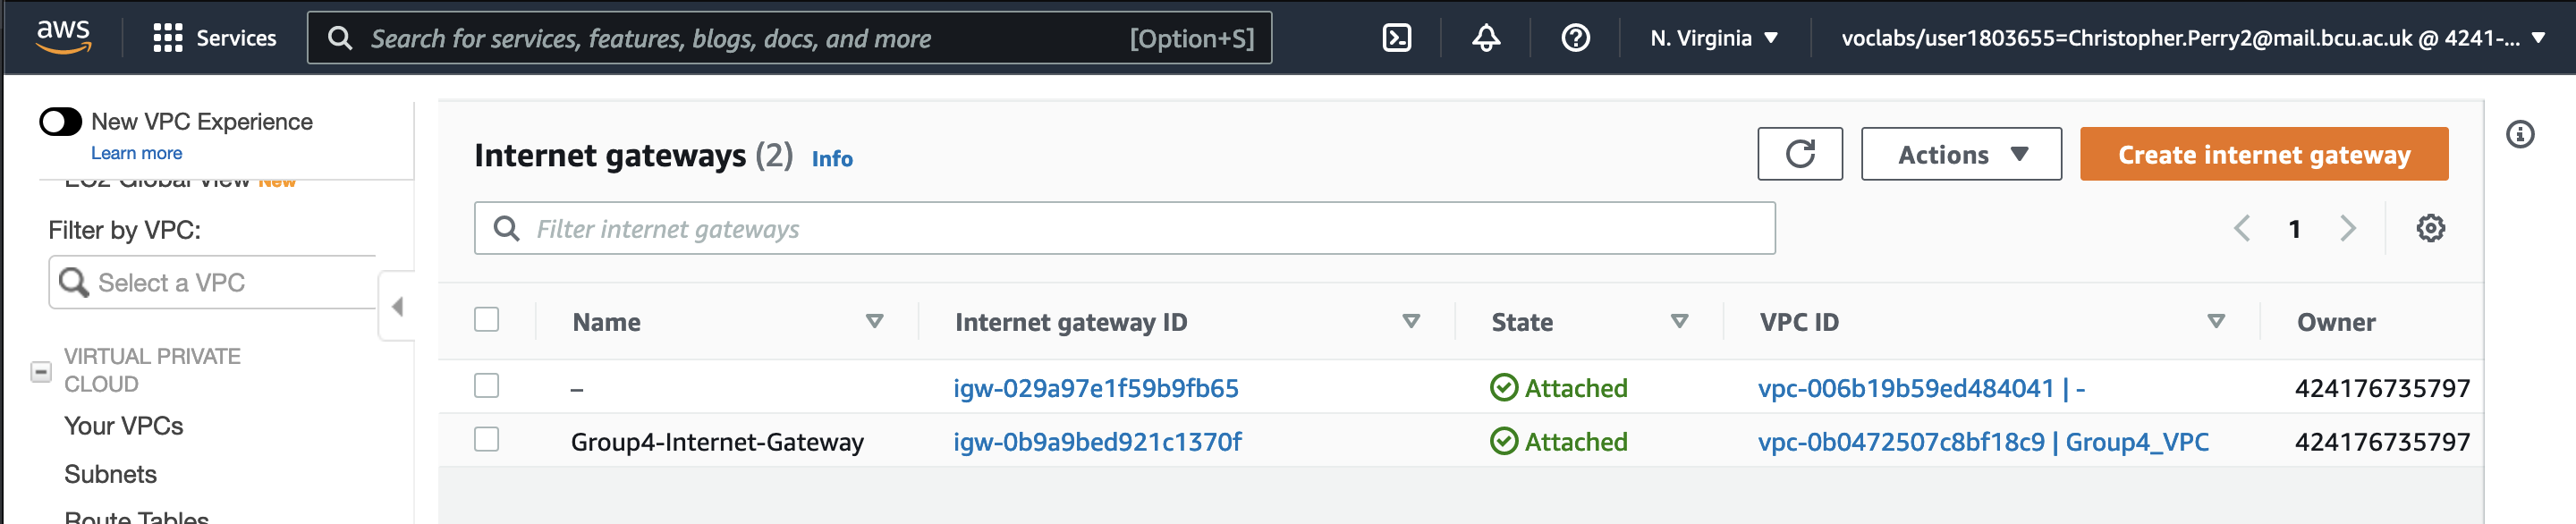
\includegraphics[width=150mm]{resources/vpc/internet-gateway-2}
    \caption{Viewing the newly created internet gateway.}
    \label{fig:internet-gateway-2}
\end{figure}

\clearpage
\section{Route Tables}\label{sec:route-tables}

The newly created VPC does not currently have a sufficient level of availability, as it is only available in one
Availability Zone - \mintinline{zsh}|us-east-1a|.
The availability of the VPC can be increased by creating a new pair of public and private subnets in a different
Availability Zone.
This is done by navigating to the Create Subnets page from the VPC Management Console.

First, to create \mintinline{zsh}|Public subnet 2|, it is required to specify a VPC ID, an Availability Zone, and an
IPv4 CIDR block for the subnet.
For this subnet, the ID of the newly created VPC is selected as the VPC ID\@.
Additionally, \mintinline{zsh}|us-east-1b| is selected as the Availability Zone and
\mintinline{zsh}|10.0.3.0/24| is selected as the IPv4 CIDR block.

\begin{figure}[!htbp]
    \centering
    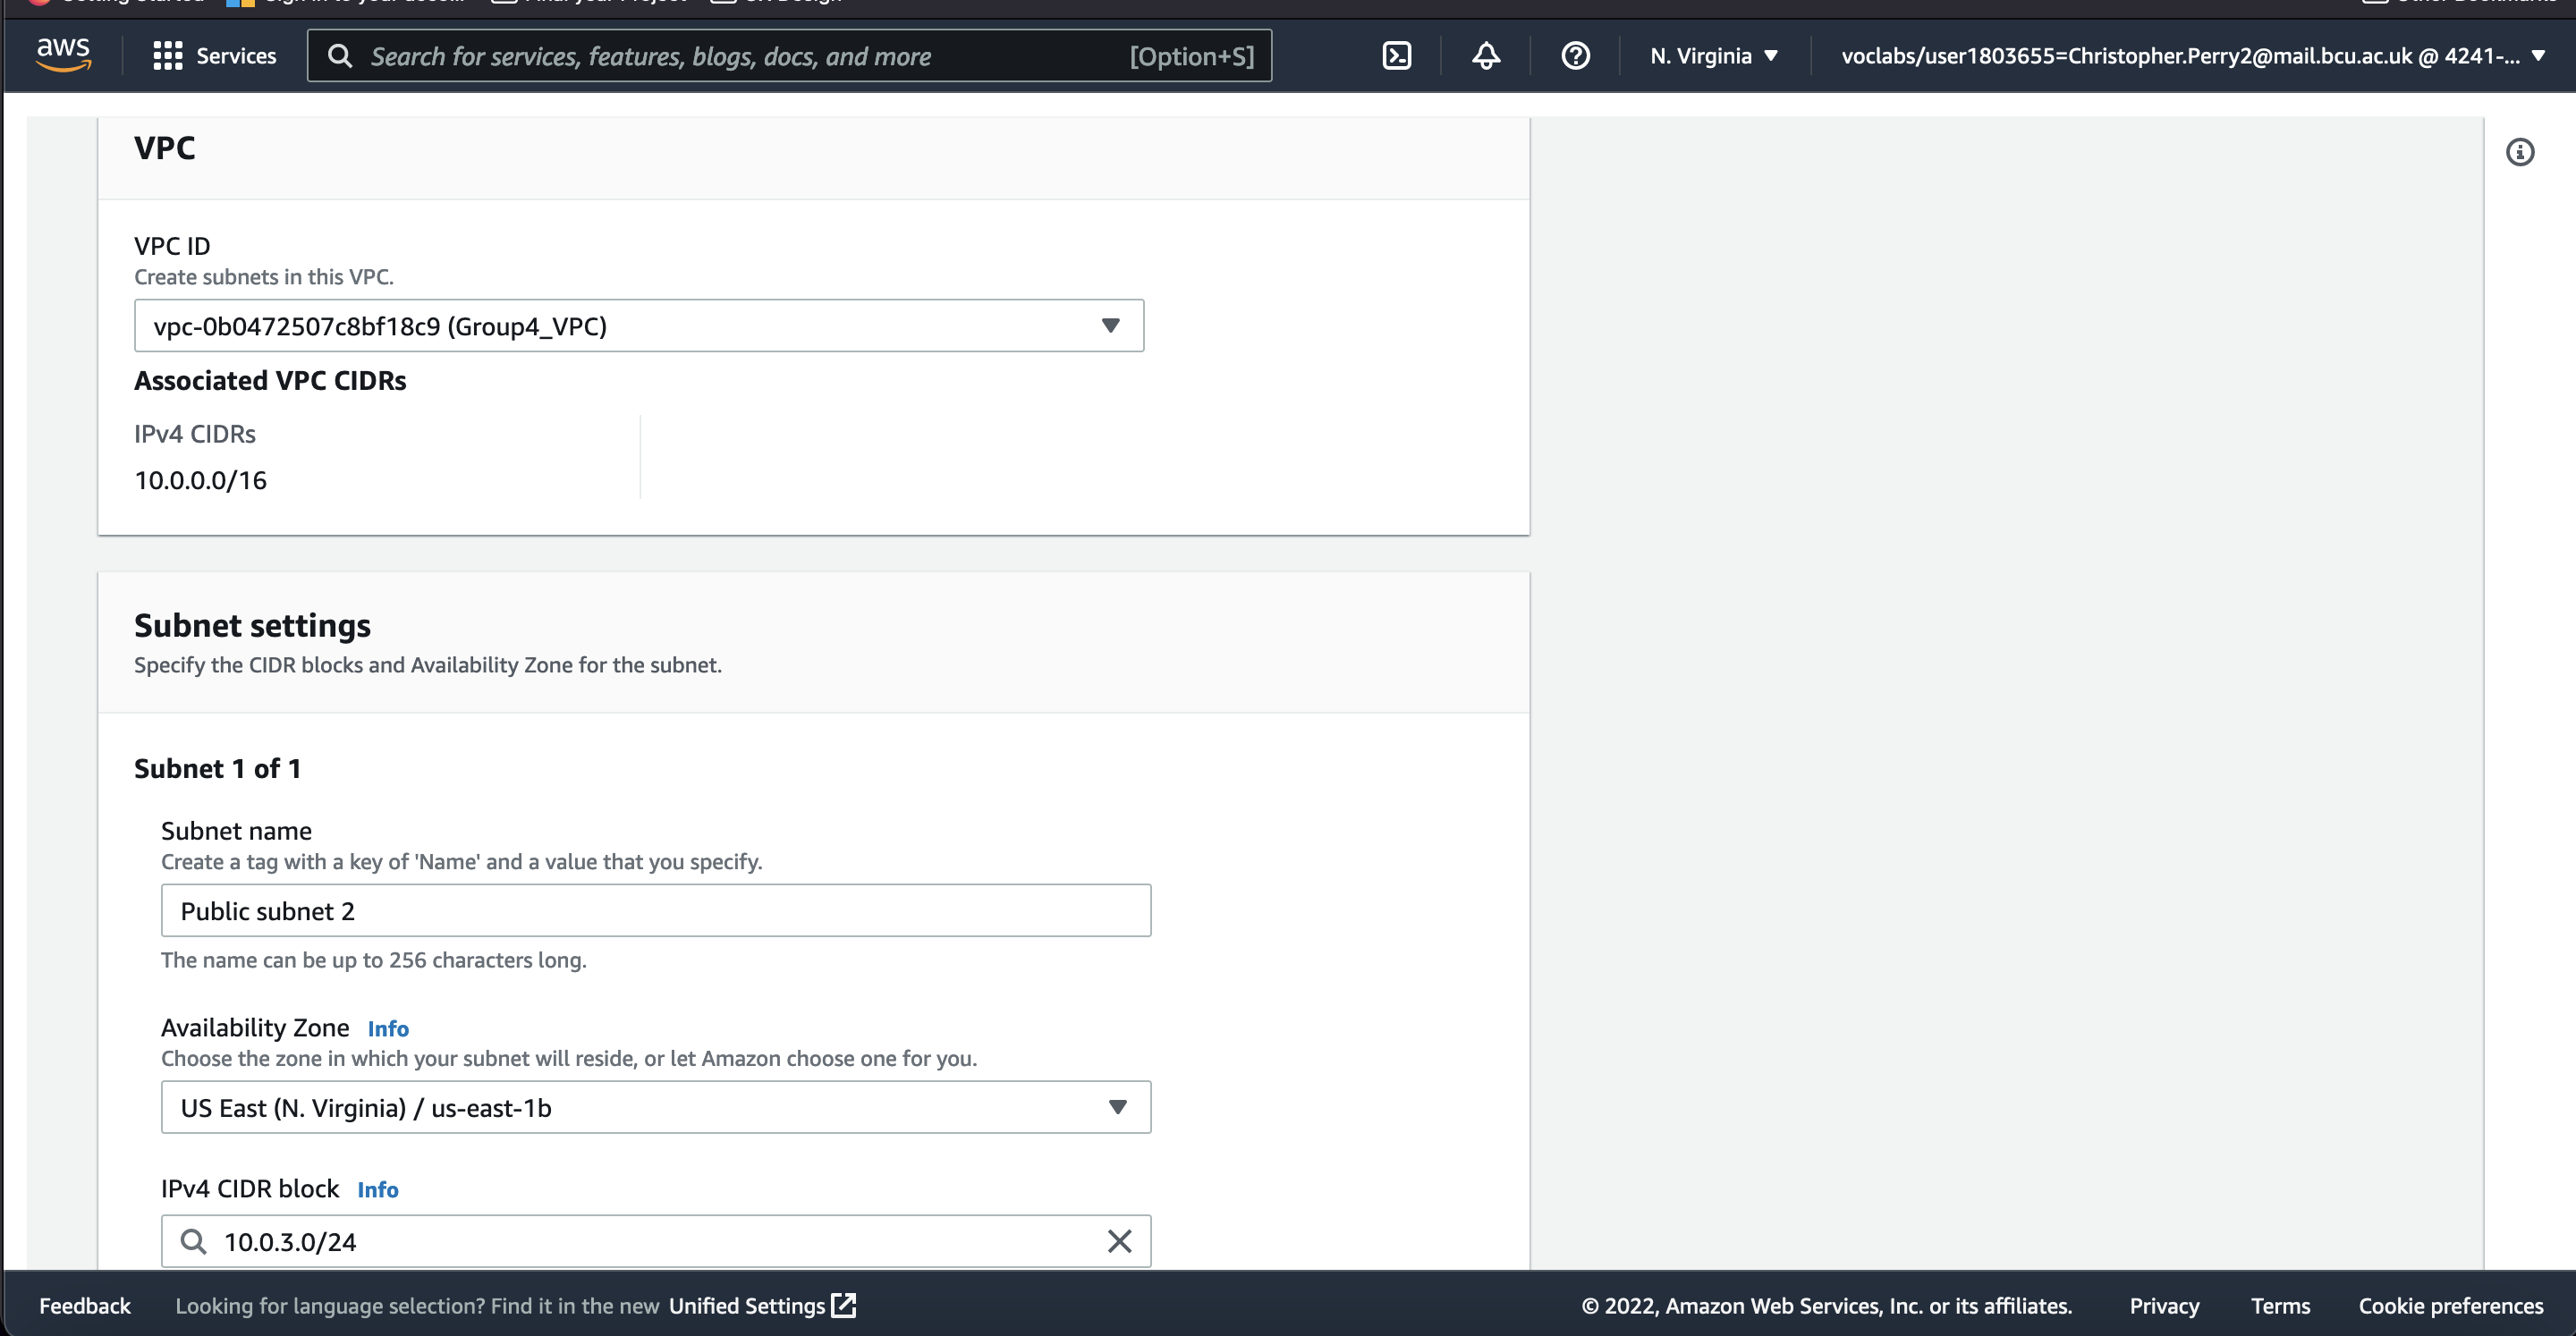
\includegraphics[width=125mm]{resources/vpc/routes/vpc-public-subnet-2}
    \caption{Creating a second public subnet.}
    \label{fig:vpc-public-subnet-2}
\end{figure}

Next, to create \mintinline{zsh}|Private subnet 2|, the ID of the newly created VPC is also selected as the VPC ID,
\mintinline{zsh}|us-east-1b| is selected as the Availability Zone and \mintinline{zsh}|10.0.4.0/24| is selected as the
IPv4 CIDR block.

\begin{figure}[!htbp]
    \centering
    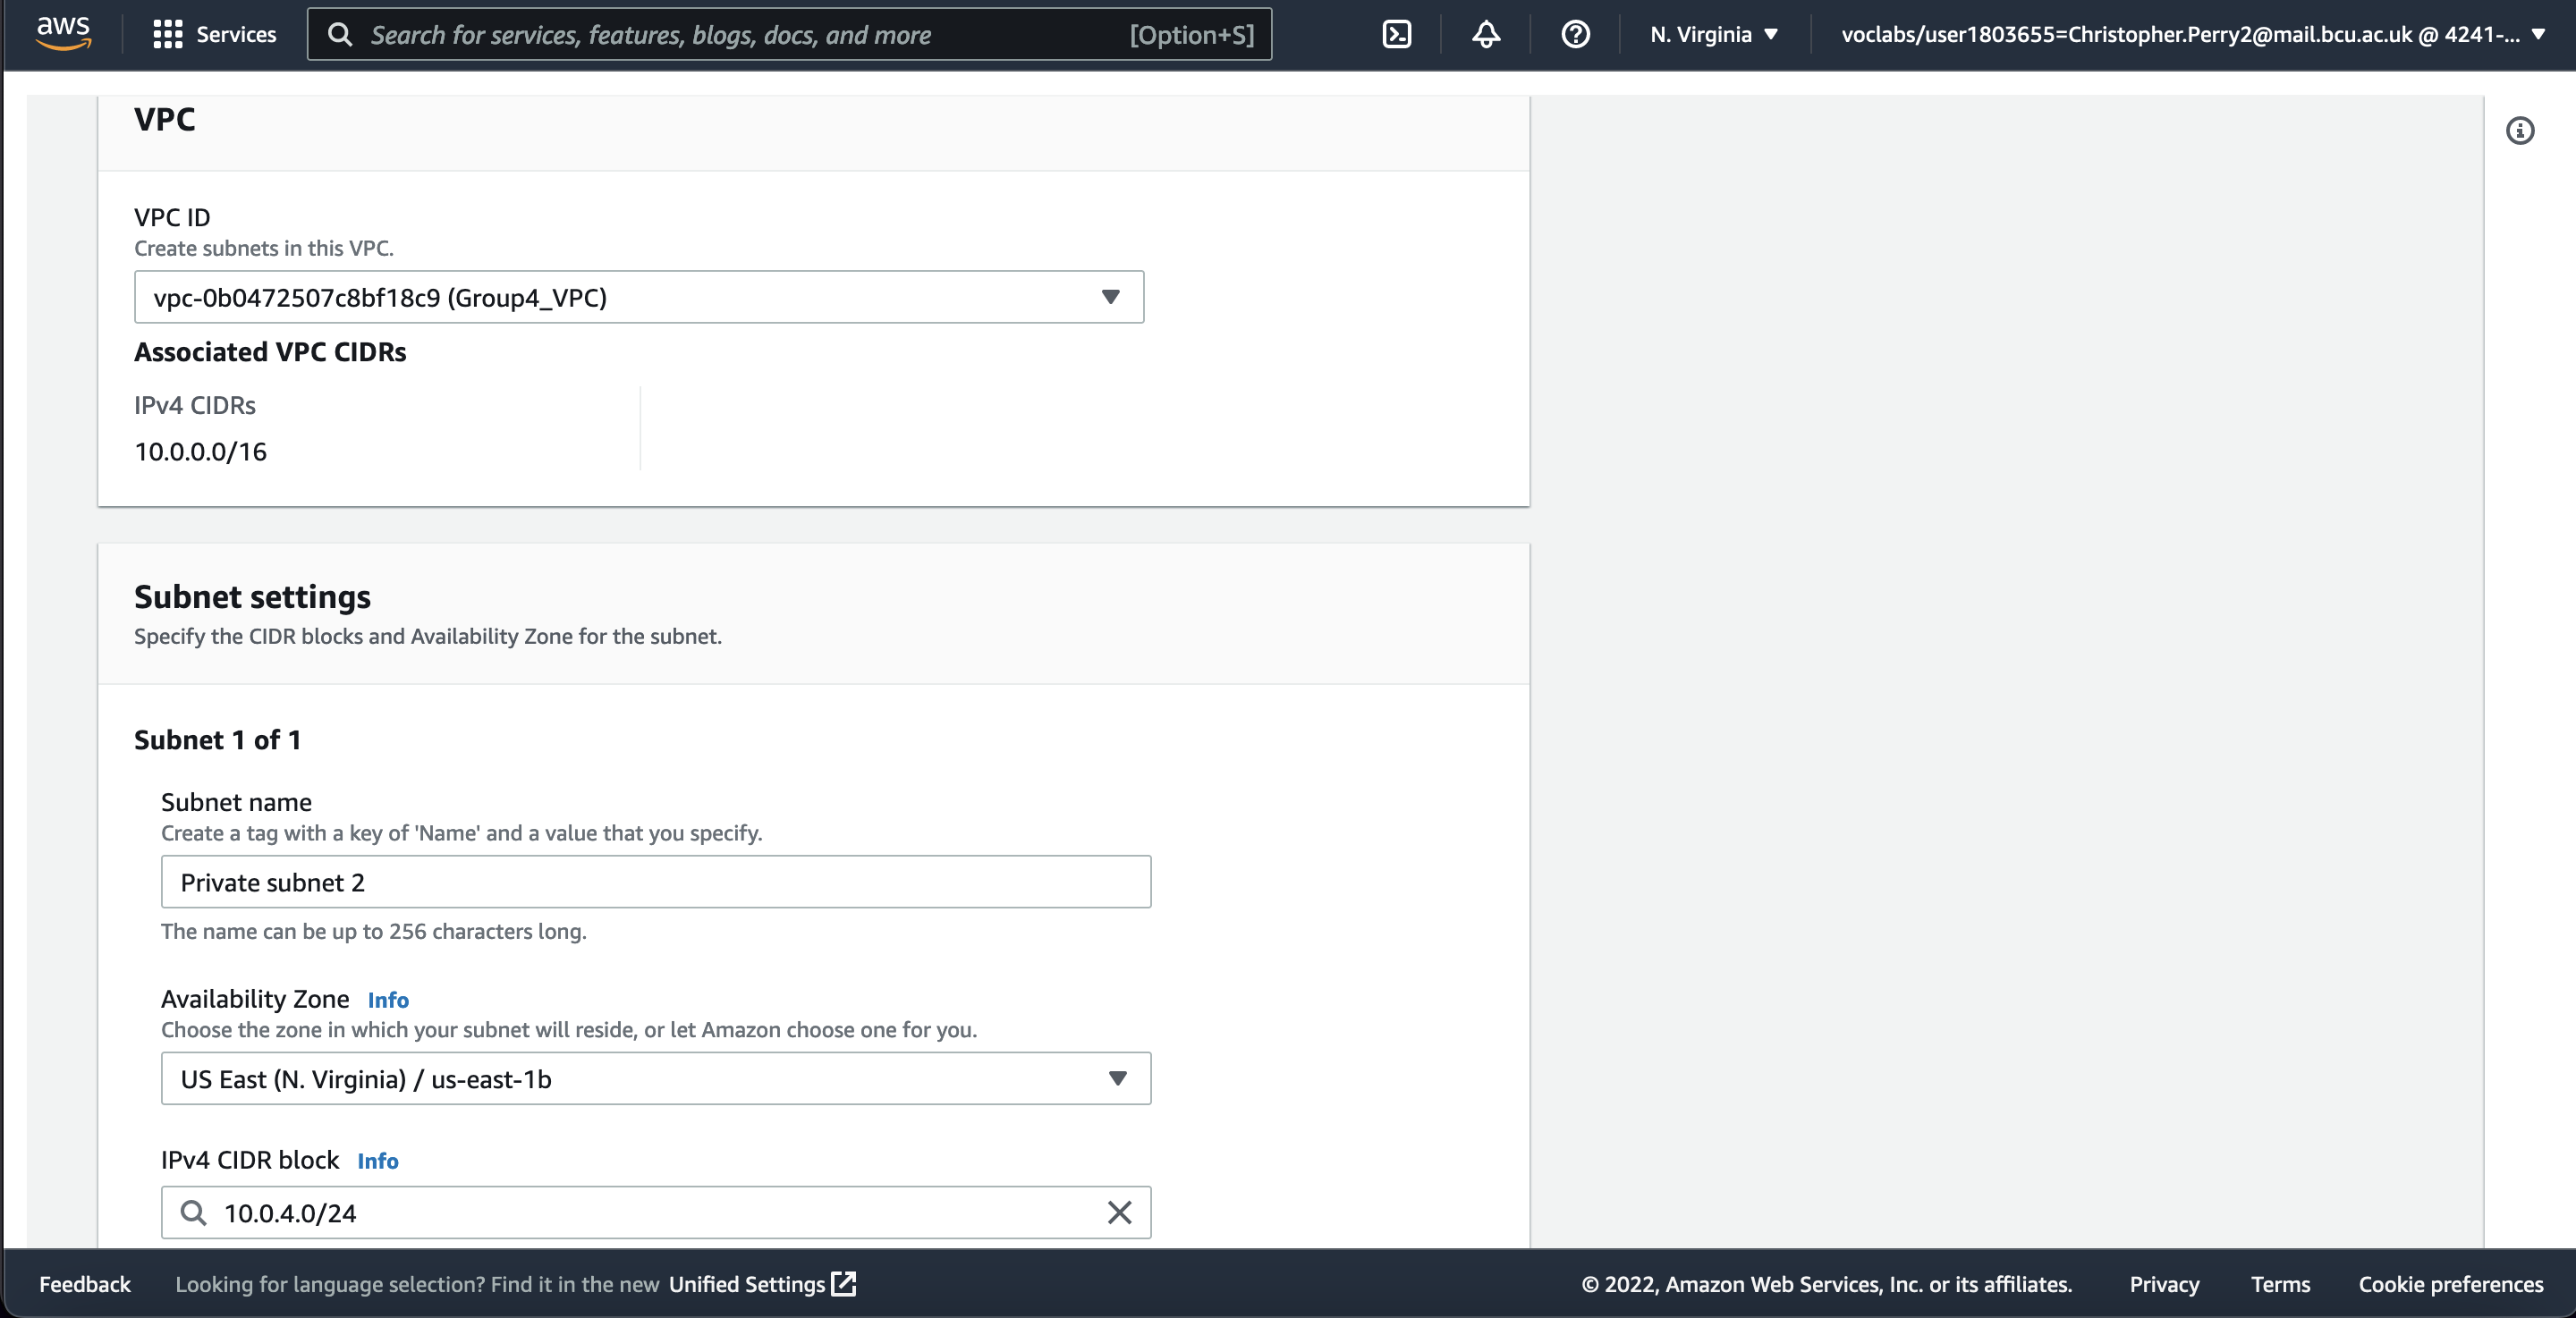
\includegraphics[width=125mm]{resources/vpc/routes/vpc-private-subnet-2}
    \caption{Creating a second private subnet.}
    \label{fig:vpc-private-subnet-2}
\end{figure}

Now the subnets can be filtered by Availability Zone and it can be seen that the two newly created subnets exist within
\mintinline{zsh}|us-east-1b| (as well as an automatically generated default subnet, which will not be used).

\begin{figure}[!htbp]
    \centering
    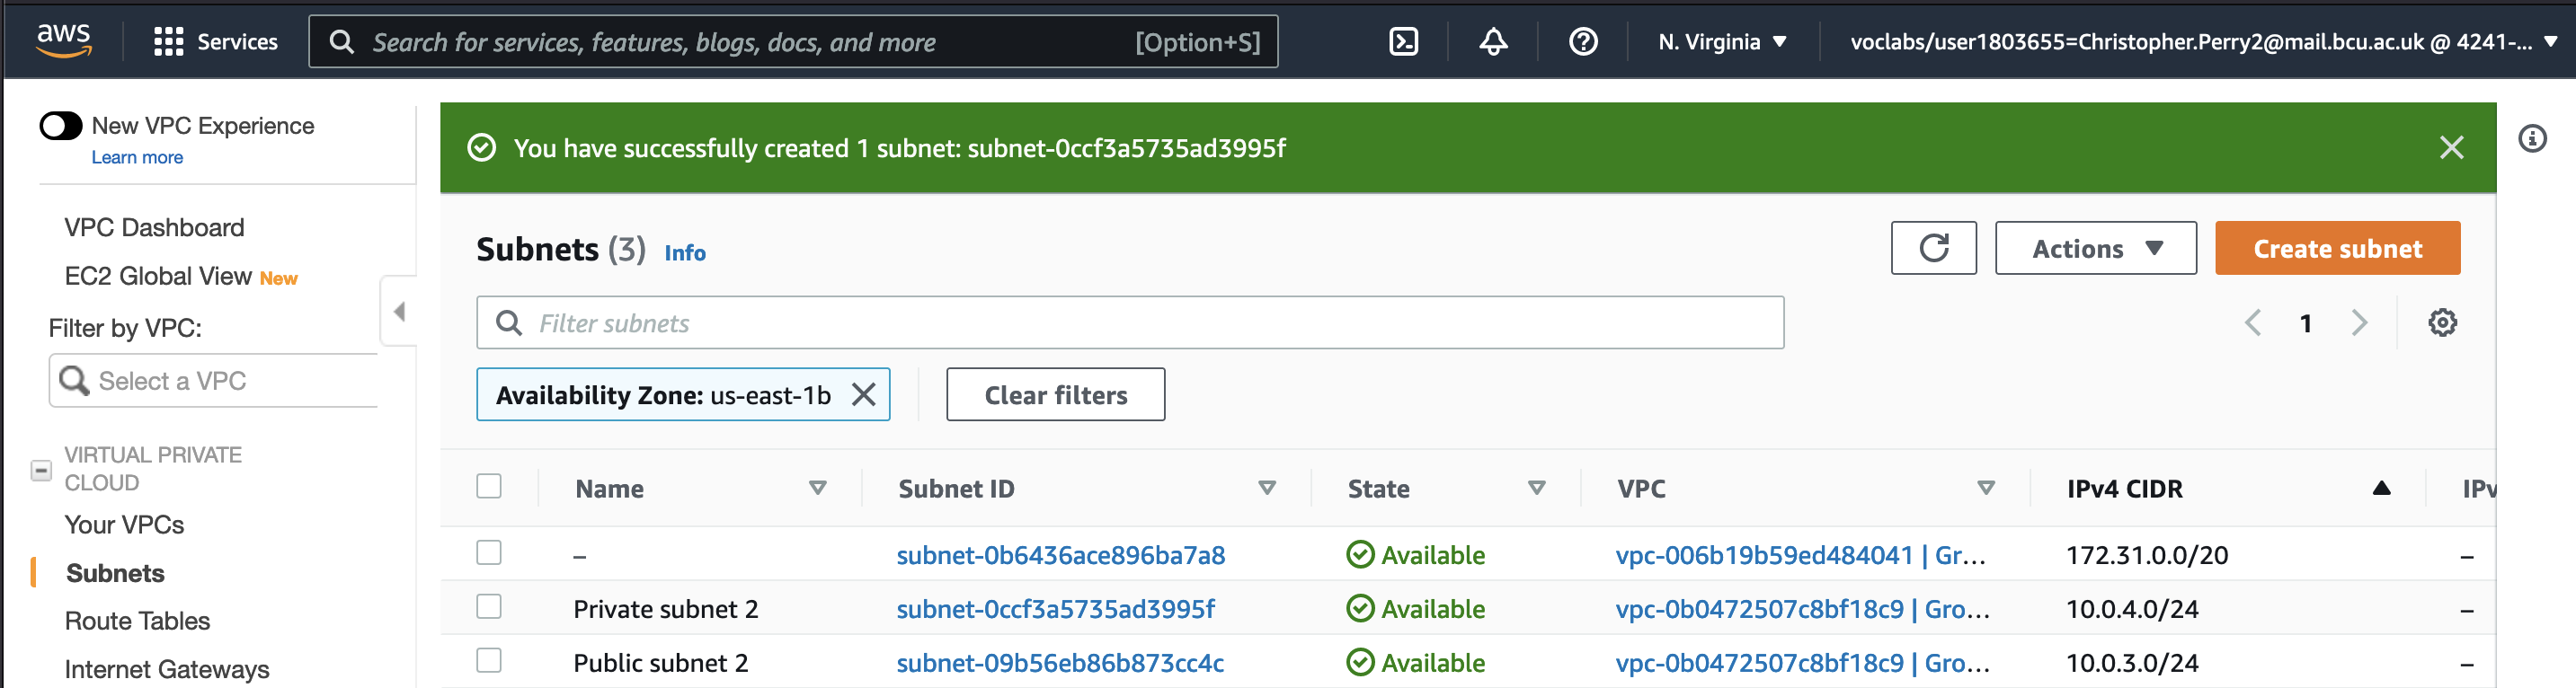
\includegraphics[width=150mm]{resources/vpc/routes/vpc-subnets-2}
    \caption{Viewing the newly created subnets.}
    \label{fig:vpc-subnets-2}
\end{figure}

After this, two routing tables must be created to link the two public subnets and the two private subnets.
The Create Route Table page can be navigated to from the VPC Management Console.
Two route tables are created, one at a time, called \mintinline{zsh}|Public route| and \mintinline{zsh}|Private route|
with the previously created VPC\@.

\begin{figure}[!htbp]
    \centering
    \subfloat{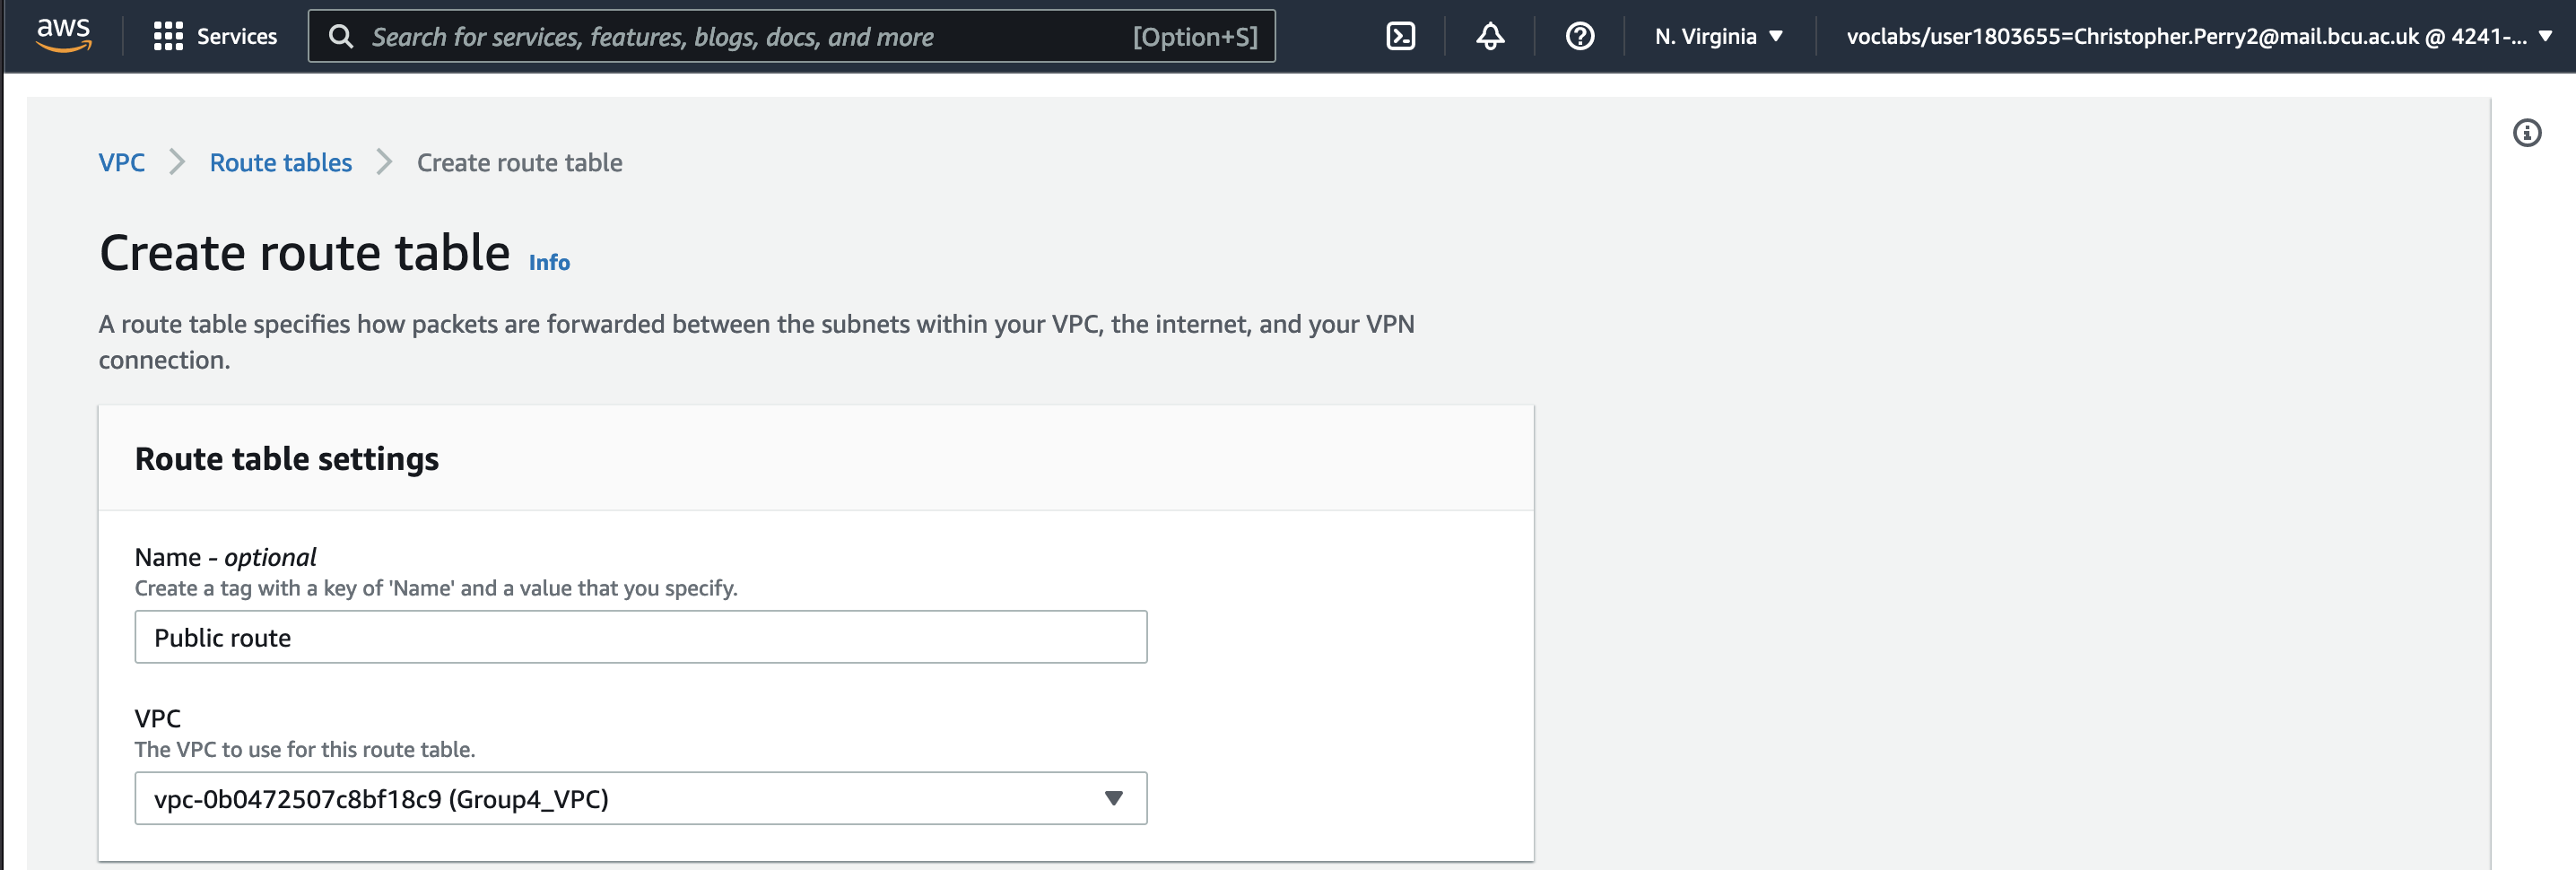
\includegraphics[width=150mm]{resources/vpc/routes/vpc-public-route}}\hfill
    \subfloat{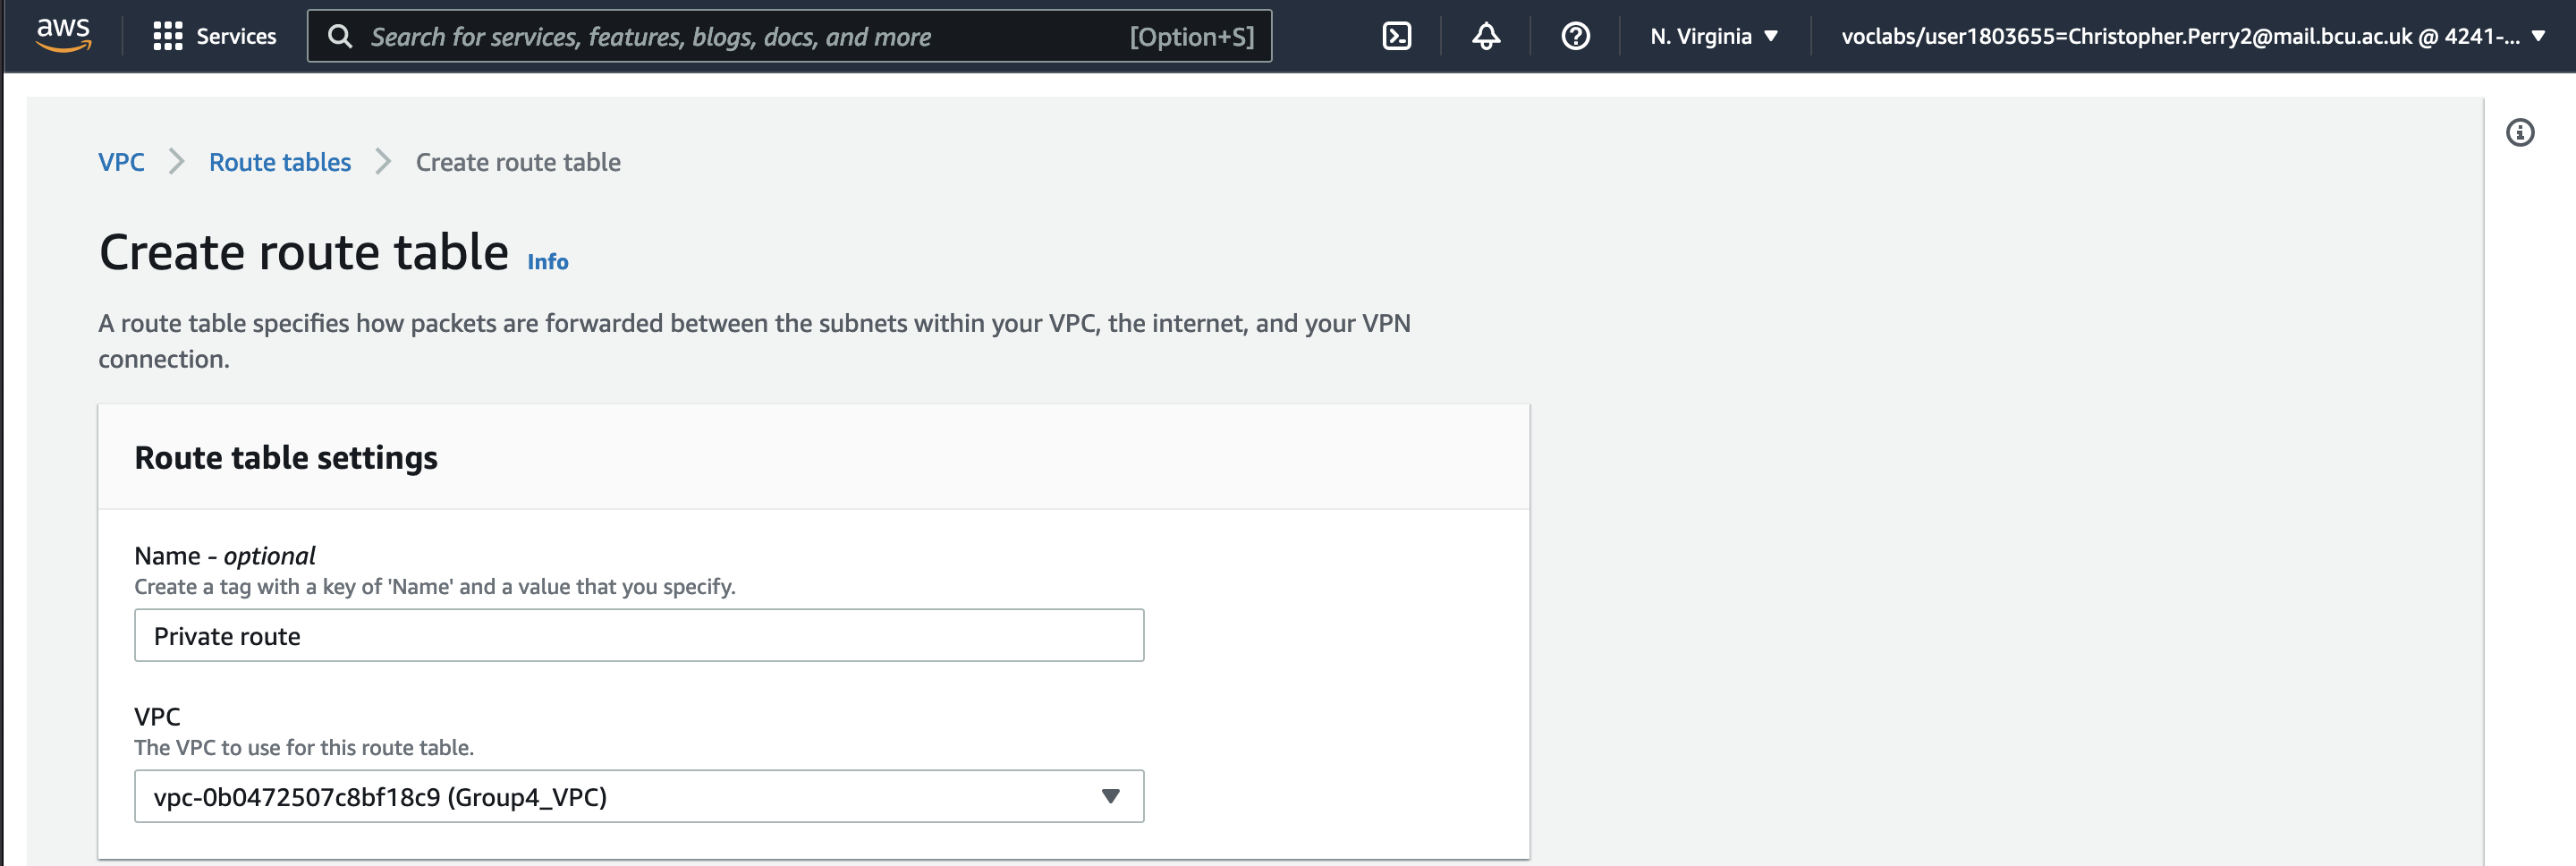
\includegraphics[width=150mm]{resources/vpc/routes/vpc-private-route}}
    \caption{Creating a public route table and a private route table.}
    \label{fig:vpc-public-route-private-route}
\end{figure}

\clearpage
Once the two route tables have been created, the public and private subnets must be associated with the corresponding
route table.
From the Route Tables page, \mintinline{zsh}|Public route| is selected, and the \textbf{Edit subnet associations} button
is clicked.
On the Edit Subnet Associations page, the two public subnets are selected, and the \textbf{Save associations} button is
clicked.
This process is then repeated for \mintinline{zsh}|Private route|.

\begin{figure}[!htbp]
    \centering
    \subfloat{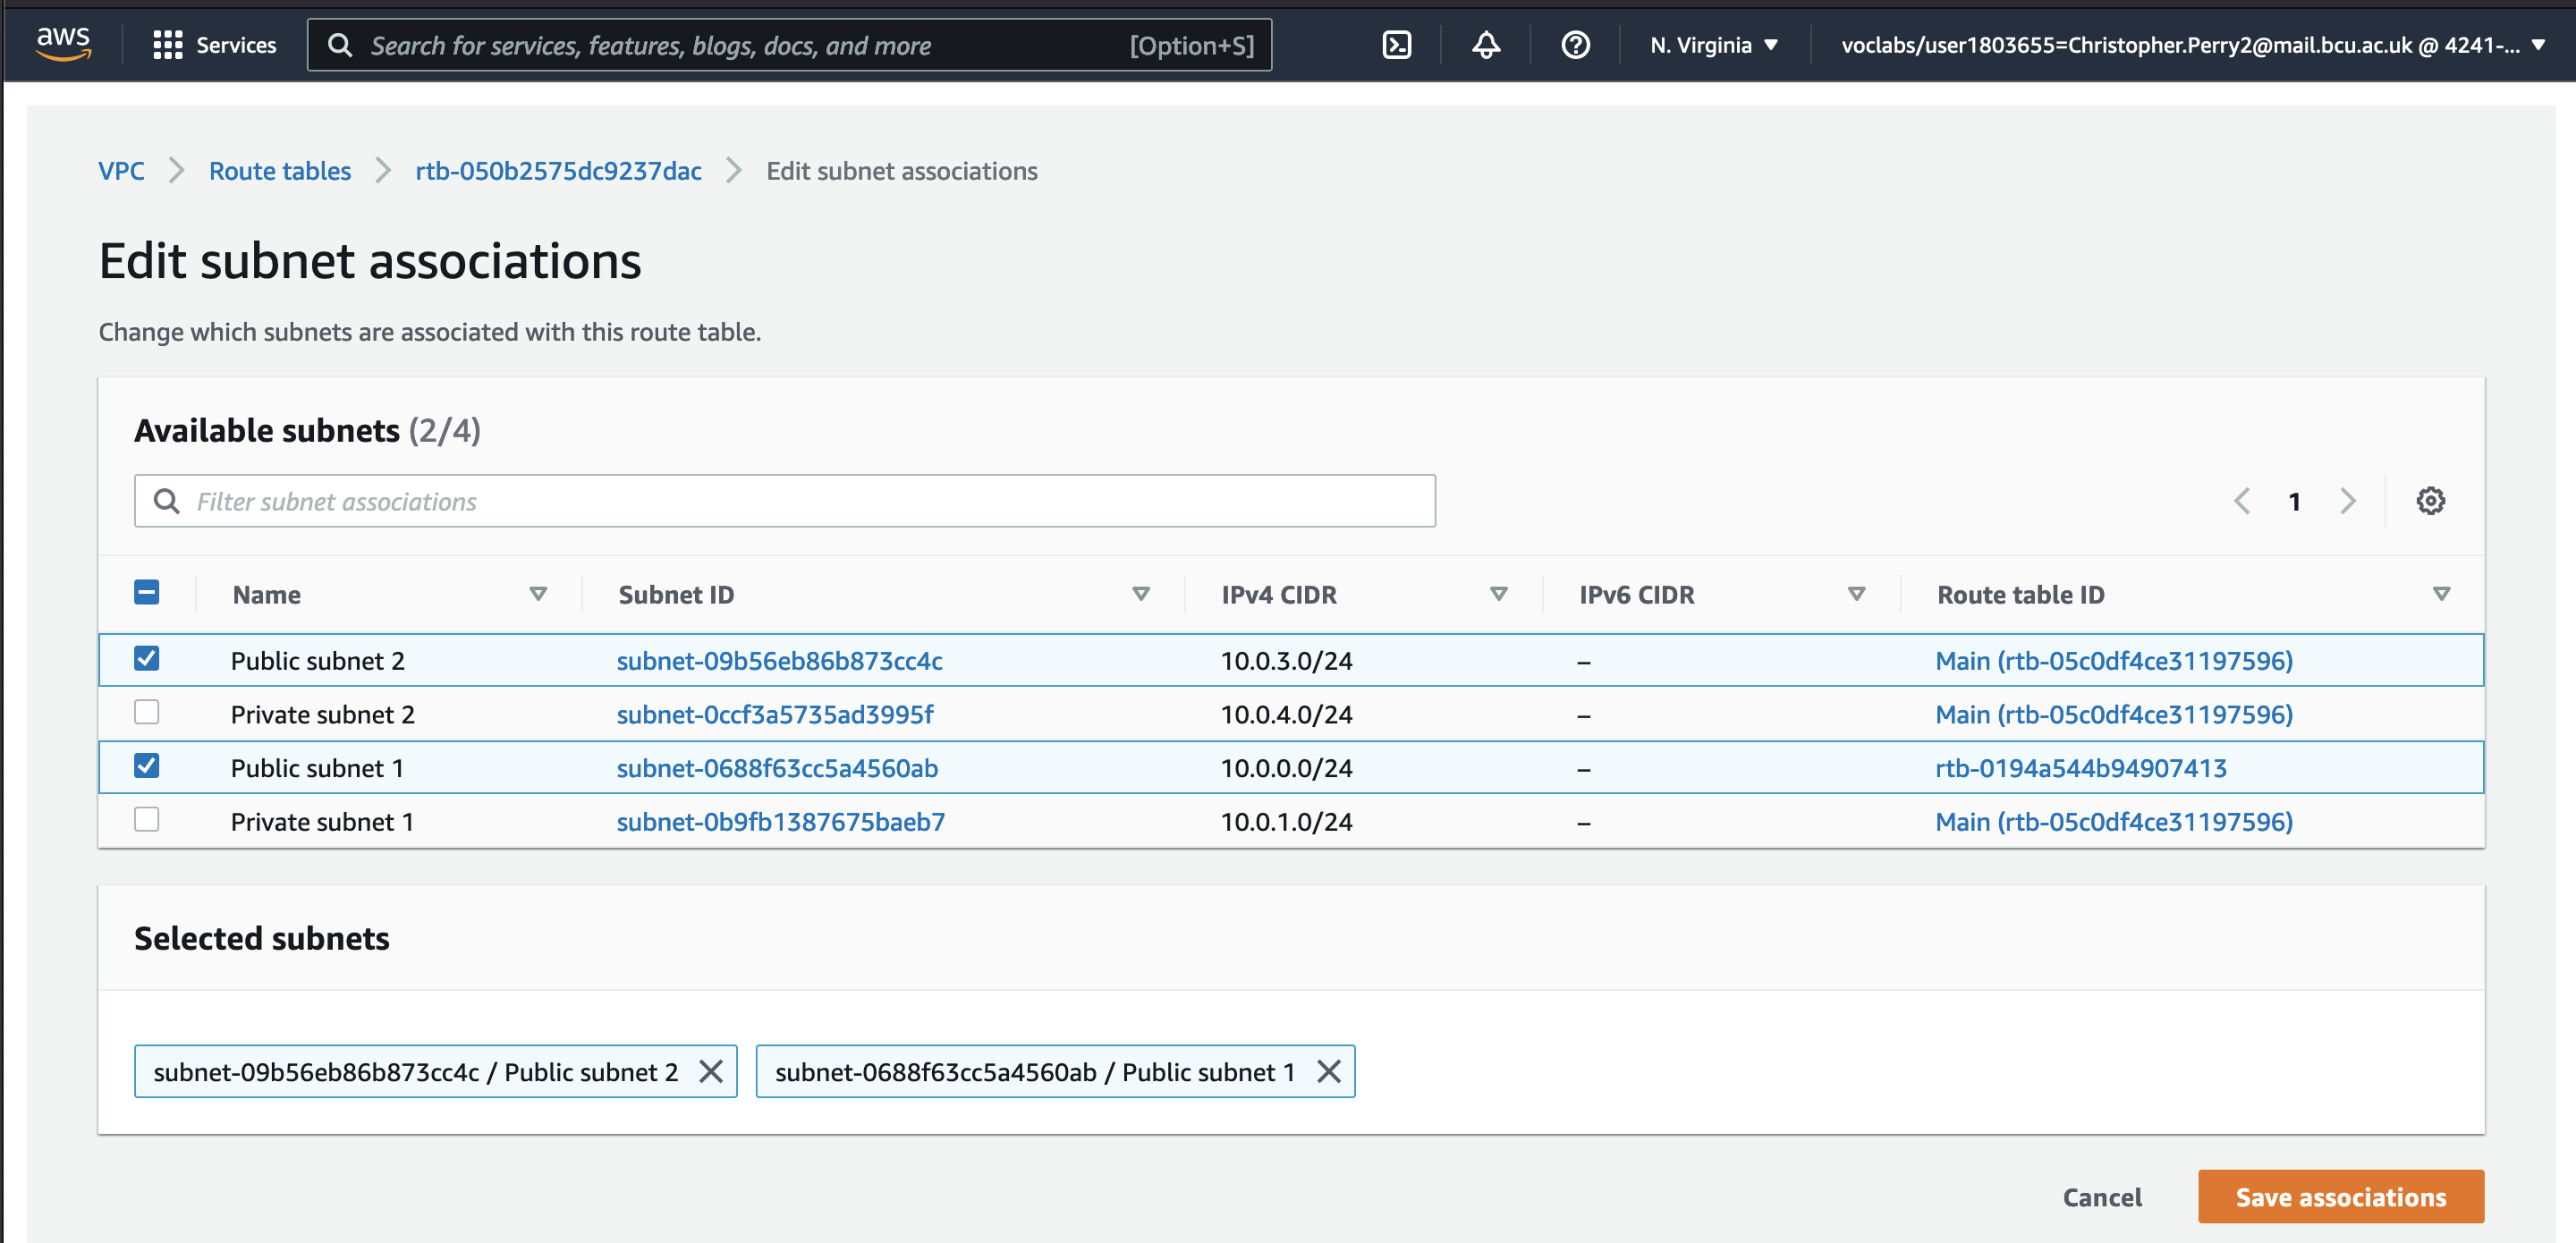
\includegraphics[width=150mm]{resources/vpc/routes/vpc-subnet-public-ass}}\hfill
    \subfloat{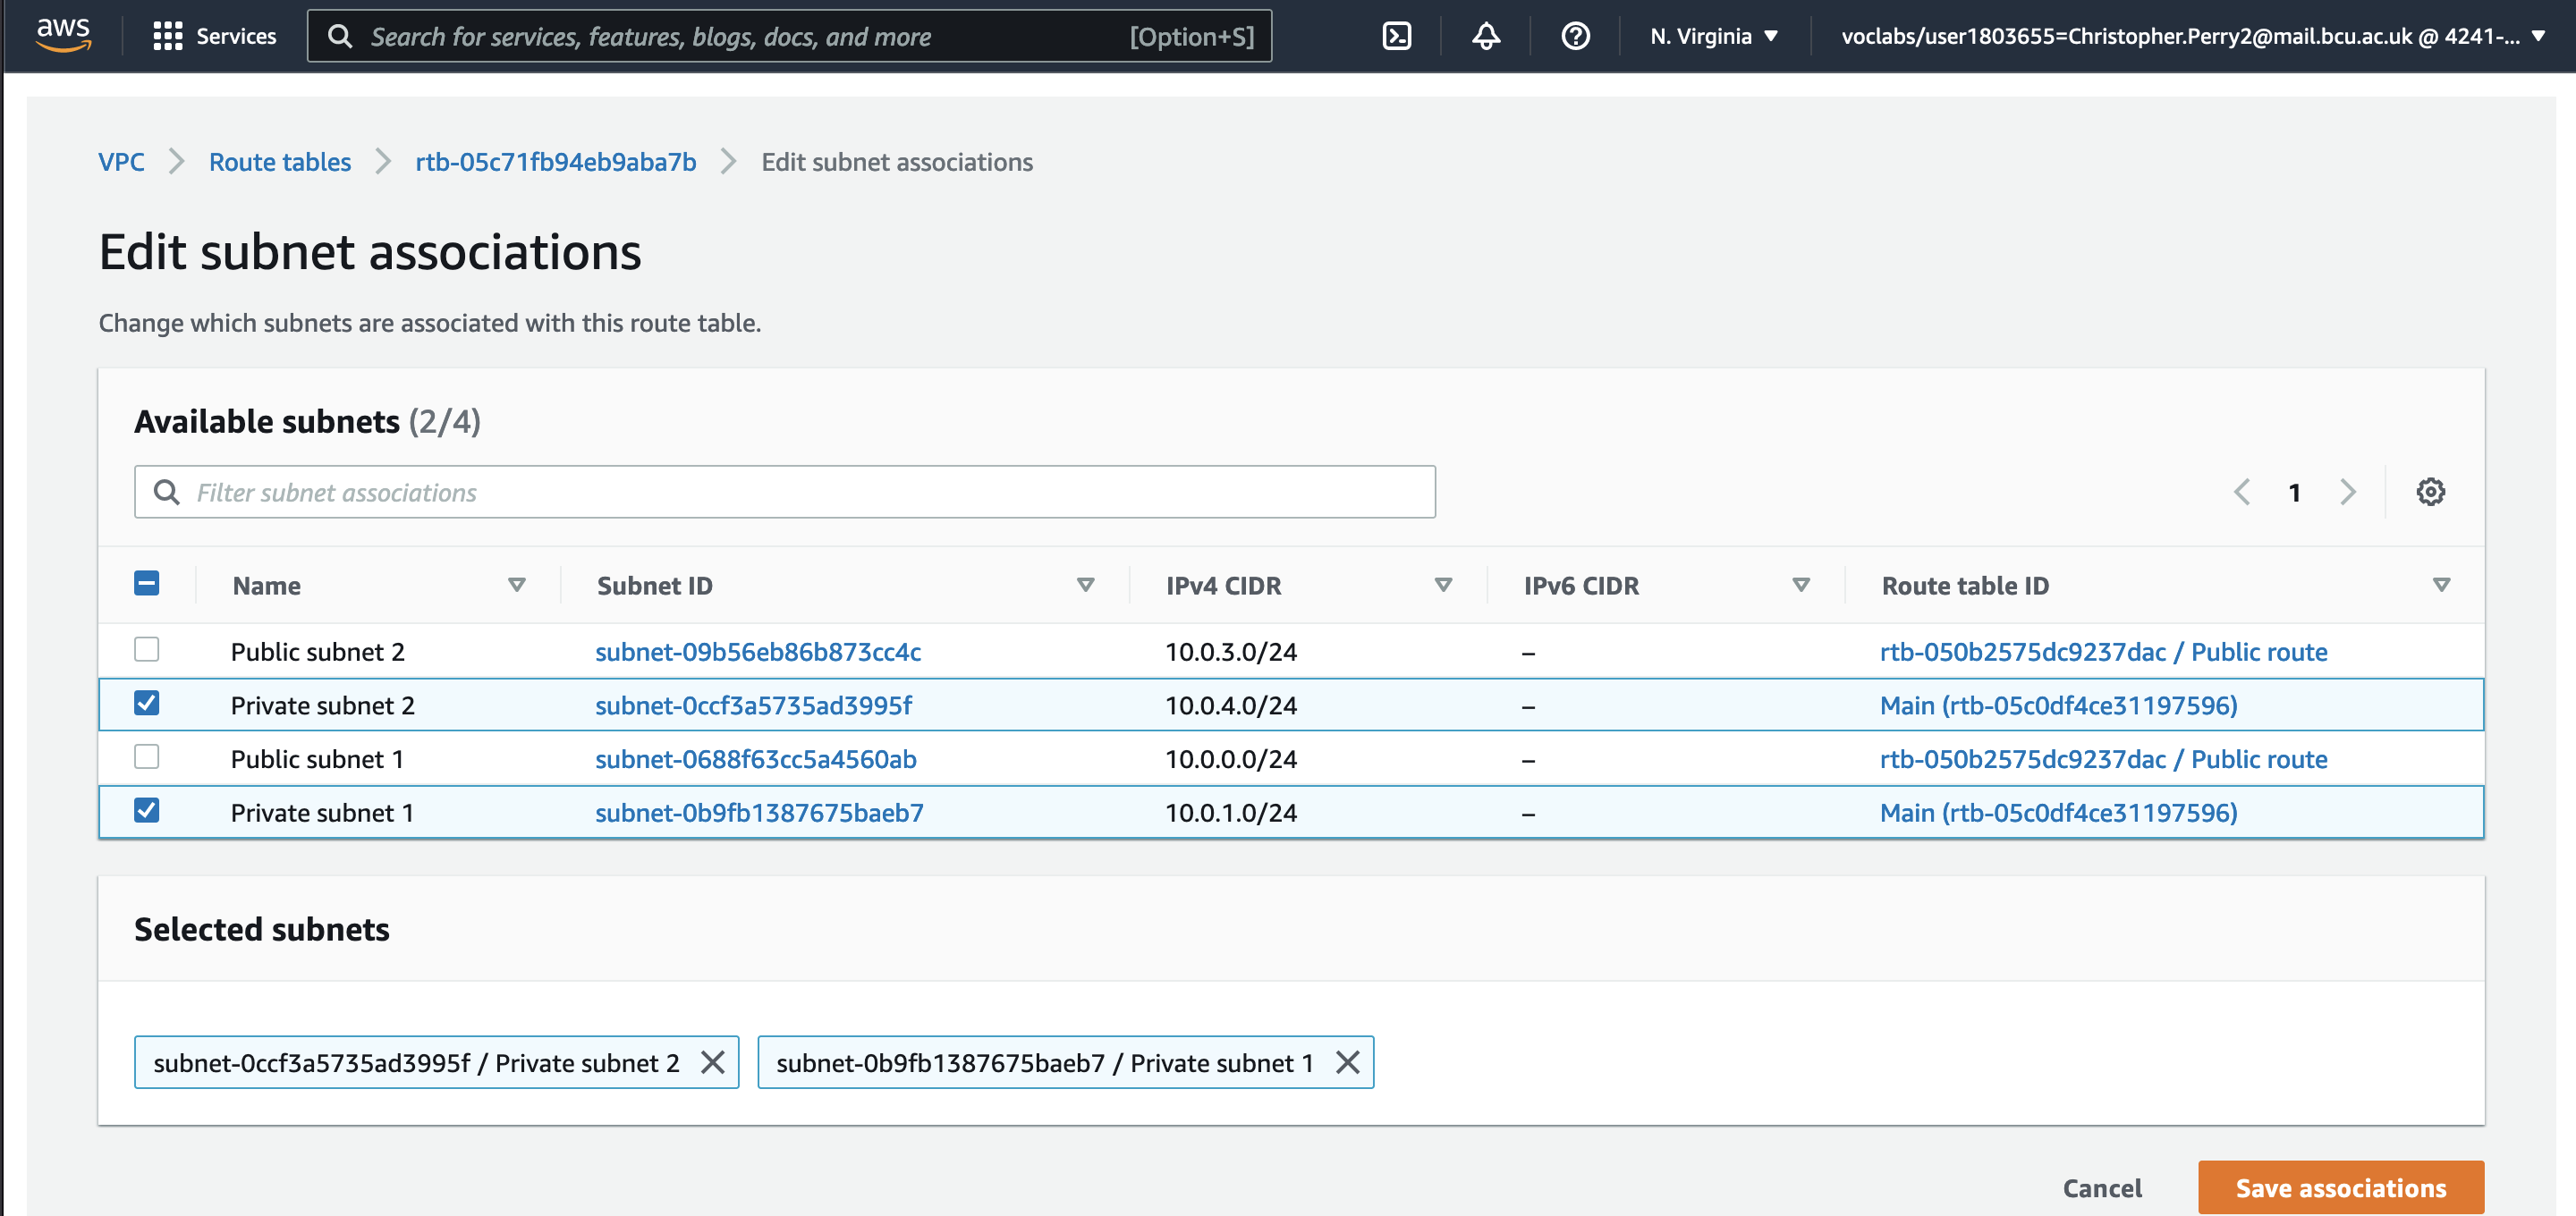
\includegraphics[width=150mm]{resources/vpc/routes/vpc-subnet-private-ass}}
    \caption{Associating the public and private subnets with the public and private route tables.}
    \label{fig:vpc-public-ass-private-ass}
\end{figure}

\clearpage
Lastly, the \mintinline{zsh}|Public route| must be updated to allow all public traffic that attempts to access the VPC
to be routed via the internet gateway.
This is done by selecting \mintinline{zsh}|Public route| and clicking the "Edit routes" Action.
On this page, click the \textbf{Add route} button and enter a destination of \mintinline{zsh}|0.0.0.0/0| and, for the target,
select the previously created internet gateway.

\begin{figure}[!htbp]
    \centering
    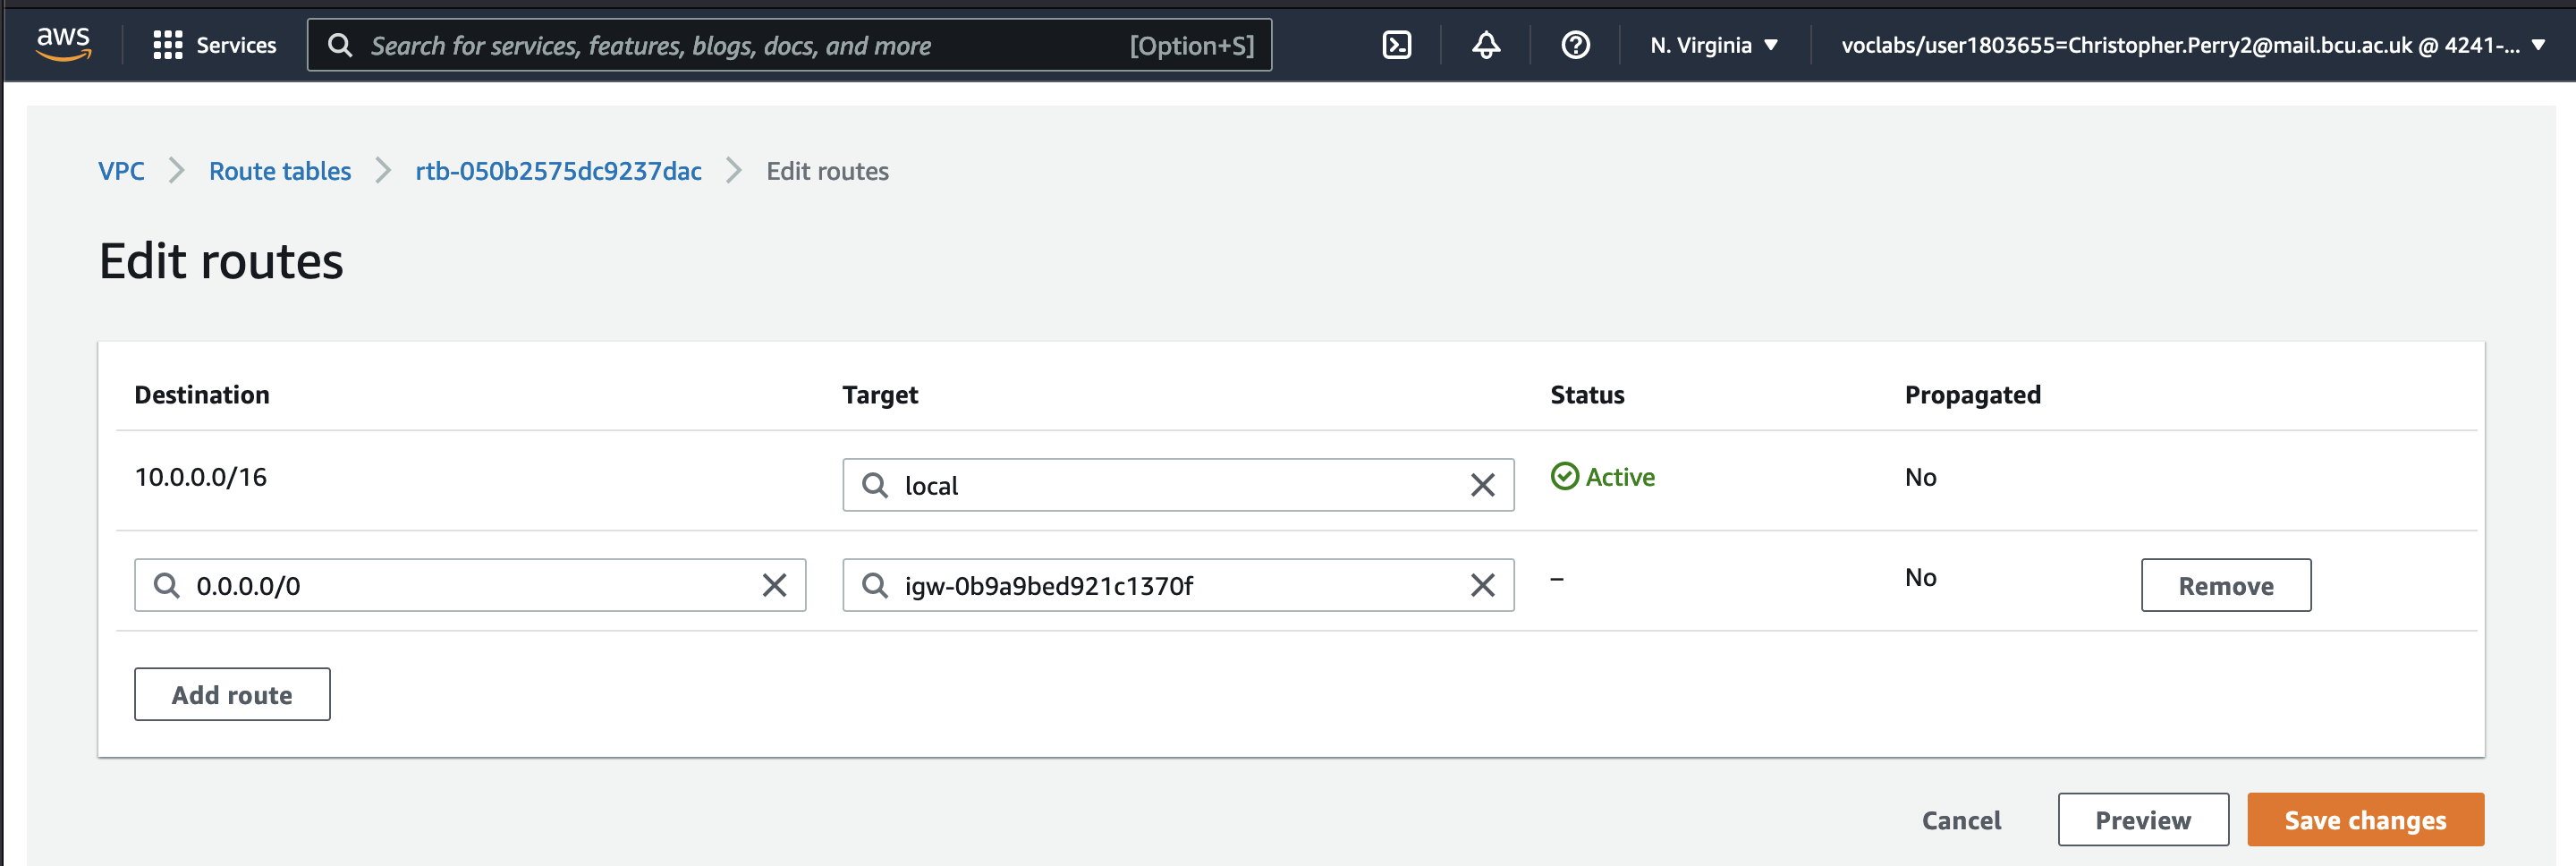
\includegraphics[width=150mm]{resources/vpc/routes/vpc-public-route-table}
    \caption{Editing the public route table.}
    \label{fig:vpc-public-route-table}
\end{figure}

Lastly, click the \textbf{Save changes} button.
This will update the route for \mintinline{zsh}|Public route|.

\begin{figure}[!htbp]
    \centering
    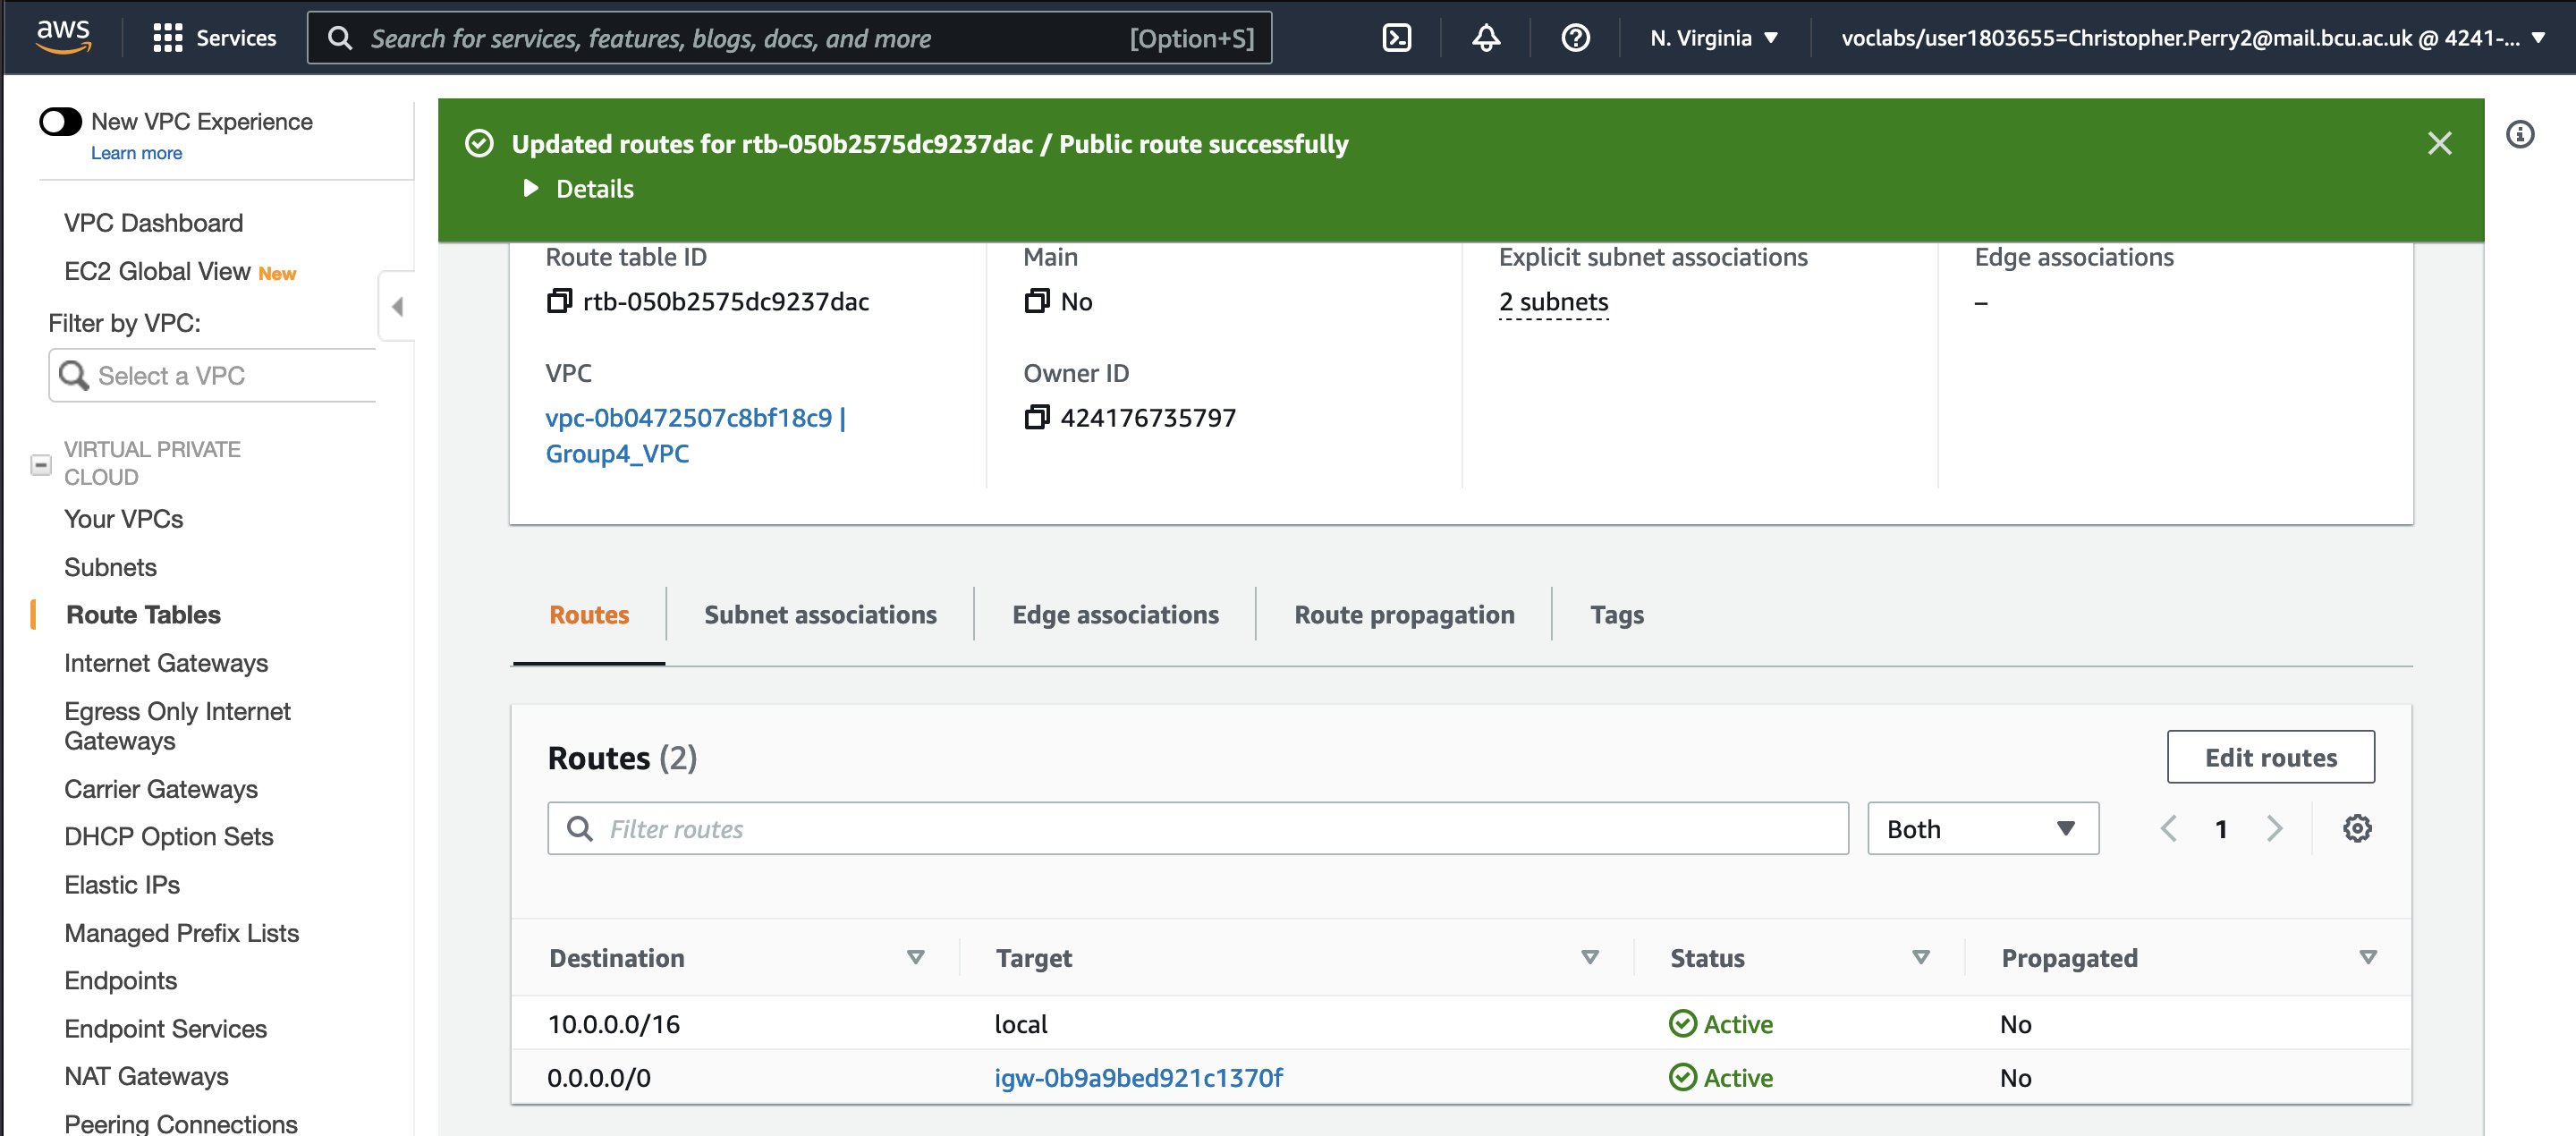
\includegraphics[width=150mm]{resources/vpc/routes/vpc-public-route-after}
    \caption{Updated public route table.}
    \label{fig:vpc-public-route-after}
\end{figure}
